\documentclass[11pt]{aghdpl}
% \documentclass[en,11pt]{aghdpl}  % praca w języku angielskim

% Lista wszystkich języków stanowiących języki pozycji bibliograficznych użytych w pracy.
% (Zgodnie z zasadami tworzenia bibliografii każda pozycja powinna zostać utworzona zgodnie z zasadami języka, w którym dana publikacja została napisana.)
\usepackage[english,polish]{babel}

% Użyj polskiego łamania wyrazów (zamiast domyślnego angielskiego).
\usepackage{polski}

\usepackage[utf8]{inputenc}

% dodatkowe pakiety

\usepackage{mathtools}
\usepackage{amsfonts}
\usepackage{amsmath}
\usepackage{amsthm}
\usepackage{hyperref}
% --- < bibliografia > ---

\usepackage[
style=numeric,
sorting=none,
%
% Zastosuj styl wpisu bibliograficznego właściwy językowi publikacji.
language=autobib,
autolang=other,
% Zapisuj datę dostępu do strony WWW w formacie RRRR-MM-DD.
urldate=iso8601,
% Nie dodawaj numerów stron, na których występuje cytowanie.
backref=false,
% Podawaj ISBN.
isbn=true,
% Nie podawaj URL-i, o ile nie jest to konieczne.
url=false,
%
% Ustawienia związane z polskimi normami dla bibliografii.
maxbibnames=3,
% Jeżeli używamy BibTeXa:
backend=bibtex
]{biblatex}

\usepackage{csquotes}
% Ponieważ `csquotes` nie posiada polskiego stylu, można skorzystać z mocno zbliżonego stylu chorwackiego.
\DeclareQuoteAlias{croatian}{polish}

\addbibresource{bibliografia.bib}

% Nie wyświetlaj wybranych pól.
%\AtEveryBibitem{\clearfield{note}}


% ------------------------
% --- < listingi > ---

% Użyj czcionki kroju Courier.
\usepackage{courier}

\usepackage{listings}
\lstloadlanguages{TeX}

\lstset{
	literate={ą}{{\k{a}}}1
           {ć}{{\'c}}1
           {ę}{{\k{e}}}1
           {ó}{{\'o}}1
           {ń}{{\'n}}1
           {ł}{{\l{}}}1
           {ś}{{\'s}}1
           {ź}{{\'z}}1
           {ż}{{\.z}}1
           {Ą}{{\k{A}}}1
           {Ć}{{\'C}}1
           {Ę}{{\k{E}}}1
           {Ó}{{\'O}}1
           {Ń}{{\'N}}1
           {Ł}{{\L{}}}1
           {Ś}{{\'S}}1
           {Ź}{{\'Z}}1
           {Ż}{{\.Z}}1,
	basicstyle=\footnotesize\ttfamily,
}

% ------------------------

\AtBeginDocument{
	\renewcommand{\tablename}{Tabela}
	\renewcommand{\figurename}{Rys.}
}

% ------------------------
% --- < tabele > ---

\usepackage{array}
\usepackage{tabularx}
\usepackage{multirow}
\usepackage{booktabs}
\usepackage{makecell}
\usepackage[flushleft]{threeparttable}

% defines the X column to use m (\parbox[c]) instead of p (`parbox[t]`)
\newcolumntype{C}[1]{>{\hsize=#1\hsize\centering\arraybackslash}X}


%---------------------------------------------------------------------------

\author{Jarosław Borzęcki}
\shortauthor{J. Borzęcki}

%\titlePL{Przygotowanie bardzo długiej i pasjonującej pracy dyplomowej w~systemie~\LaTeX}
%\titleEN{Preparation of a very long and fascinating bachelor or master thesis in \LaTeX}

\titlePL{Ewaluacja i integracja algorytmów wizyjnych stosowanych w pojazdach autonomicznych z użyciem symulatora jazdy samochodem}
\titleEN{Evaluation and integration of vision algorithms used in autonomous vehicles with the use of a driving simulator}


\shorttitlePL{Ewaluacja i integracja algorytmów wizyjnych stosowanych w pojazdach
autonomicznych z użyciem symulatora jazdy samochodem} % skrócona wersja tytułu jeśli jest bardzo długi
\shorttitleEN{Evaluation and integration of vision algorithms used in autonomous vehicles with the use of a driving simulator}

\thesistype{Praca dyplomowa magisterska}
%\thesistype{Master of Science Thesis}

\supervisor{dr inż. Tomasz Kryjak}
%\supervisor{Marcin Szpyrka PhD, DSc}

\degreeprogramme{Automatyka i robotyka}
%\degreeprogramme{Computer Science}

\date{2019}

\department{Katedra Automatyki i robotyki}
%\department{Department of Applied Computer Science}

\faculty{Wydział Elektrotechniki, Automatyki,\protect\\[-1mm] Informatyki i Inżynierii Biomedycznej}
%\faculty{Faculty of Electrical Engineering, Automatics, Computer Science and Biomedical Engineering}

\acknowledgements{Serdecznie dziękuję wszystkim.}


\setlength{\cftsecnumwidth}{10mm}

%---------------------------------------------------------------------------
\setcounter{secnumdepth}{4}
\brokenpenalty=10000\relax

\begin{document}

\titlepages

% Ponowne zdefiniowanie stylu `plain`, aby usunąć numer strony z pierwszej strony spisu treści i poszczególnych rozdziałów.
\fancypagestyle{plain}
{
	% Usuń nagłówek i stopkę
	\fancyhf{}
	% Usuń linie.
	\renewcommand{\headrulewidth}{0pt}
	\renewcommand{\footrulewidth}{0pt}
}

\setcounter{tocdepth}{2}
\tableofcontents
\clearpage
\chapter*{ }
\section*{Streszczenie pracy}


W ramach niniejszej pracy stworzono system, który w połączeniu z symulatorem jazdy umożliwia testowanie algorytmów wizyjnych stosowanych w zaawansowanych systemach wspomagania kierowcy i pojazdach autonomicznych.
W części teoretycznej przedstawiono szereg algorytmów wizyjnych, zarówno tych korzystających z tradycyjnego przetwarzania obrazów cyfrowych, a także głębokouczonych sieci neuronowych.
Po krótkiej analizie dostępnych symulatorów jazdy wybrano Euro Truck Simulator 2 czeskiego studia SCS Software.
Jego przewaga nad innym programami dostępnymi na rynku polega na dużych możliwościach modyfikacji oraz interfejsu programistycznego udostępnianego przed twórców.
W ramach pracy stworzona została aplikacja w języku Python 3.7.
Jej architektura jest wieloprocesowa, co oznacza, że każda z głównych funkcjonalności: przechwytywanie i analiza obrazu, generowanie 
sterowania i opcjonalne wyświetlanie wyników są realizowane równolegle, każda w osobnym procesie.
Pozwoliło to na zwiększenie wydajności całego systemu, gdyż należy mieć na uwadze fakt, że oprócz działającej aplikacji na stacji roboczej jest uruchomiony symulator jazdy.
Działanie systemu zaprezentowano poprzez zaimplementowanie i uruchomienie 4 przykładowych algorytmów wizyjnych: wyszukiwanie linii oddzielających pasy ruchu, wykrywania znaków drogowych i sygnalizacji świetlnej oraz detekcja pojazdu poprzedzającego.
Cele pracy zostały osiągnięte, a~ponadto wskazano dalsze kierunki rozwoju systemu.



\section*{Abstract}

The thesis describes a system, which together with a~driving simulator enables to test vision algorithms used in Advanced Driver Assistance Systems (ADAS).
In first, theoretical part, there several vision algorithms have been presented, both based on traditional image processing and deep convolutional neural networks.
After short analysis of the available driving simulators, the Euro Truck Simulator 2 created by Czech studio SCS Software was chosen.
It's advantage over other solutions is that the user is able to modify it in a variety of ways. 
Moreover there is an API attached to simulator.
The main application was developed with use of Python 3.7.
It has a multiprocess architecture, that means every of the main functionalities (capturing and analysing a video frame, generating control vector and optional results display) are executed concurrently, every in single sub-process.
This allowed to boost the application's performance. 
An important thing to consider is that both, the developed system and driving simulator run on the same computer.
An operation of the developed system was presented by implementing four example vision algorithms: lane, traffic sign, traffic light and preceding vehicle detection. 
All goals of the thesis have been achieved, and some improvements for future works proposed.

\chapter{Wstęp}
\section{Cele i założenia}
Niniejsza praca powstała w celu stworzenia faplikacji umożliwiającej testowanie algorytmów wizyjnych za pomocą symulatora ciężarówki, która mogłaby być wykorzystana w ramach zajęć z Systemów Wizyjnych w Pojazdach Autonomicznych prowadzonych w ramach kierunku Automatyka i Robotyka na Akademii Górniczo-Hutniczej.

\section{Istniejące systemy}
Aplikacje służące do testowania algorytmów wizyjnych są używane w przemyśle. Obecnie produkowane samochody są wyposażone w pewne asysty, które bazując na widoku z kamery pomagają prowadzić samochód. Testowanie tych algorytmów jest niezwykle istotne, ponieważ niewykrycie błędu prowadzi do katastrofalnych skutków, w tym potencjalnej śmierci człowieka. Niewystarczające testowanie algorytmów w komercyjnym samochodzie Tesla 3 doprowadziło do śmiertelnego wypadku, ponieważ systemy jazdy autonomicznej nie wykryły poprawnie naczepy ciężarówki.


\chapter{Systemy wizyjne w pojazdach autonomicznych}
Współczesne pojazdy autonomiczne wykorzystują w szerokim zakresie systemy wizyjne do analizy otoczenia. Jednym z pierwszych zastosowań algorytmów cyfrowego przetwarzania obrazów była detekcja pasa ruchu, która nie służyła do sterowania samochodem, lecz miała za zadanie wspomagać kierowcę w sytuacjach zmęczenia lub utraty koncentracji. Wraz z rozwojem technologii pojazdów autonomicznych, zaawansowanie systemów wizyjnych rosło od wspomnianej kontroli pasa ruchu, poprzez rozpoznawanie znaków drogowych i świateł ulicznych, na detekcji pieszych kończąc. Ważnym elementem o którym należy wspomnieć, że istotne znaczenie, oprócz algorytmów detekcji, ma sposób interpretacji danych odczytanych z otoczenia. W kolejnych podrozdziałach zostaną opisane algorytmy wizyjne, które mogłyby być zastosowane w systemach w pojazdach autonomicznych. 

\section{Poziomy autonomiczności}

Całość systemów, które wspomagają kierowcę w trakcie jazdy nazwano ADAS (Advanced Driver Assistance Systems). Aby usystematyzować  i podzielić poziom wpływu systemów na jazdę wprowadzono poziomy autonomiczności jazdy.

\begin{figure}
  \centering
  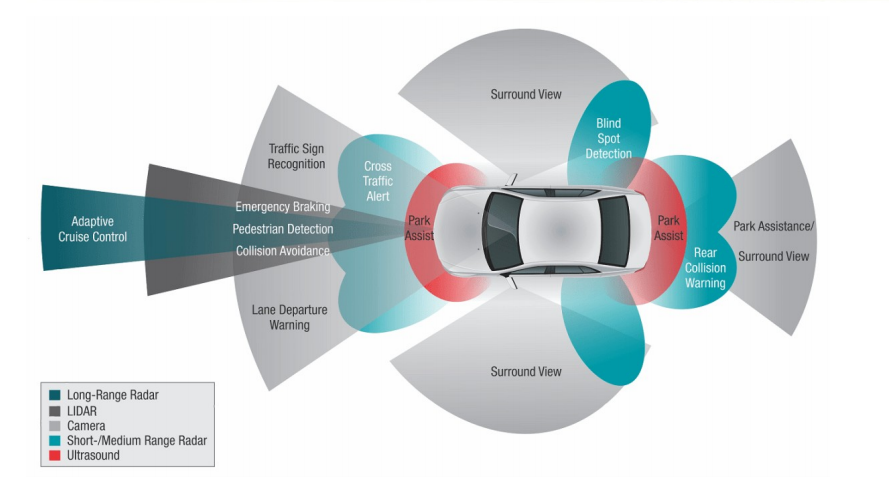
\includegraphics[width=13cm]{img/systemy_autonomiczne_ogolnie.png}
  \caption{Ogólny schemat kamer i radarów we współczesnych pojazdach autonomicznych\cite{S1}}
  \label{fig:kamery_i_radary}
  % https://aindustryreports.com/2019/05/23/advanced-driver-assistance-system-sensor-market-technological-innovations-in-north-america-to-boost-regional-market-attractiveness-through-2026/
\end{figure}

Na rysunku \ref{fig:kamery_i_radary} daje się zauważyć znaczna liczba kamer i radarów wspomagająca kierowcę. Powszechną techniką jest stosowanie redundancji w krytycznych systemach, co jest regulowane poprzez normy ADAS (Advanced Driver Assistance Systems)

\subsection{Poziom zerowy - brak autonomiczności}
Obecnie większość samochodów na drodze zawiera się w tym poziomie. Człowiek wpływa na jazdę, chociaż mogą pojawiać się proste systemy, które mogą pomóc kierowcy np. system awaryjnego hamowania. Dopóki nie wpływa on na tor jazdy, nie jest to system autonomiczny. Innym przykładem jest system ABS, który również nie jest systemem, który zapewniałby autoomiczność pojazdowi. Służy on poprawie bezpieczeństwa i jego działanie opiera się tylko na odczycie danych z czjujników niezależnie od aktualnej sytuacji na drodze i wokół pojazdu.

\subsection{Poziom pierwszy - asysty kierowcy}
Jest to najniższy poziom autonomiczności. Auto posiada pojedynczy system wspomagania kierowcy taki jak sterowanie lub przyspieszanie (tempomat). Adaptacyjny tempomat, czyli system, który zachowuje bezpieczny dystans od poprzedzającego pojazdu kwalifikuje się jako poziom pierwszy, ponieważ człowiek kontroluje pozostałe aspekty jazdy samochodem takie jak kierowanie i hamowanie.

\subsection{Poziom drugi - częściowa automatyzacja jazdy samochodem}
Oznacza zaawansowane asysty kierowcy. Samochód może sam kontrolować zarówne sterowanie i przyspieszanie oraz hamowanie. Jest w stanie jechać samodzielnie, lecz wymaga ciągłej obecności kierowcy za kierownicą, który może w każdej chwili przejąć kontrolę nad samochodem. Obecnie stosowane systemy jazdy autonomicznej takie jak np. Tesla Autopilot kwalifikują się jako poziom drugi.

\begin{figure}
  \centering
  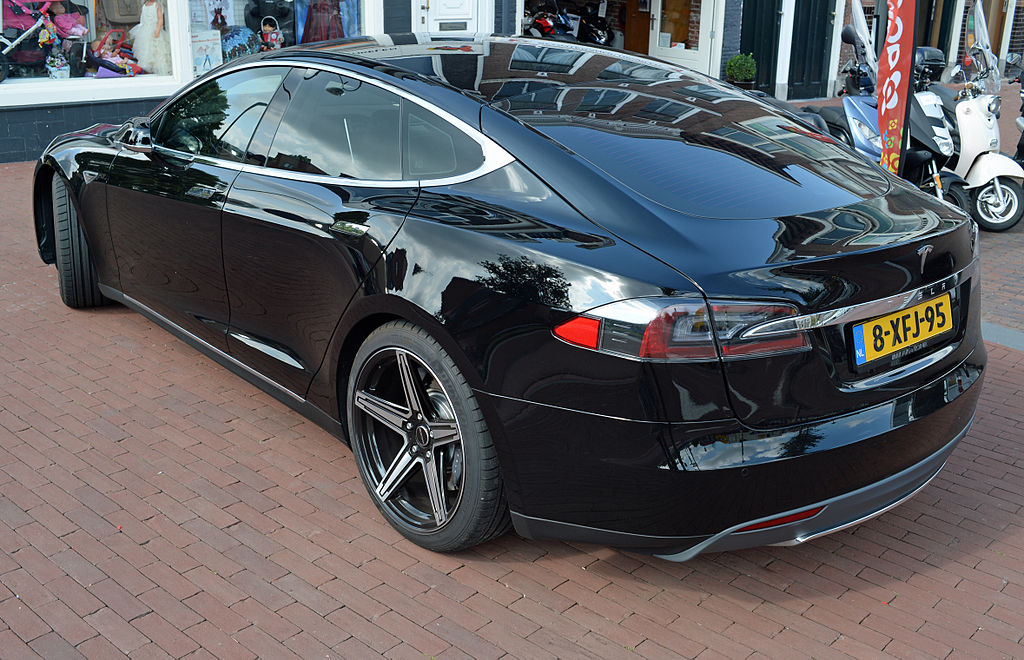
\includegraphics[width=12cm]{img/tesla.jpg}
  \caption{Tesla Model S - pierwszy samochód z drugim poziomem zaawansowania systemów wspomagania kierowcy (\textit{źródło: Wikipedia})}
  \label{fig:teslas}
  % https://pl.wikipedia.org/wiki/Tesla_Model_S#/media/Plik:2014_Tesla_Motors_Model_S_(rear_view)_Netherlands.jpg
\end{figure}

\subsection{Poziom trzeci}
Różnica w stosunku do poziomu drugiego jest subtelna. Samochód posiada możliwość detekcji otaczającego go środowiska i na podstawie zgromadzonych informacji samodzielnie podejmować decyzje. System jest jednak wciąż zależny od człowieka, który musi pozostać czujny i być w stanie zareagować, gdy system nie będzie w stanie podjąć decyzji. W 2019r. Audi wprowadziło model A8, który zapowowiadano jako pierwszy samochód poziomu trzeciego. System Traffic Jam Pilot bazując na danych z lidaru oraz kamer zapewniał autonomiczną jazdę w korkach. Problemem okazało się nieprzygotowanie prawne. W Stanach Zjednoczonych stosowanie tego systemu było zabronione, więc samochód w okrojonej wersji sprzedawano jako pojazd autonomiczny drugiego poziomu. W Europie samochód pojawił się z zaimplementowaną funkcjonalnością asystenta jazdy w korku.

\subsection{Poziom czwarty}
Poziom czwarty zapewnia to czego brakowało w niższych poziomach, a więc może interweniować jeśli coś pójdzie nie tak (np. nagły wypadek, pęknięcie opony). Te samochody nie wymagają akcji w człowieka w znakomitej większości sytuacji, jednak człowiek zawsze jest w stanie przejąć kontrolę. Podobnie jak w poziomie trzecim problemem okazały się ograniczenia prawne. Samochody te mogą z reguły poruszać się na ograniczonym obszarze. Obecnie w fazie testów są samochody takie jak Waymo lub NAVYA

\subsection{Poziom piąty - pełna autonomia}
Samochody nie wymagają uwagi człowieka. Najprawdopobniej nie będą wyposażone w kierownicę ani pedały. Będą w stanie jechać gdziekolwiek i robić to co jest w stanie zrobić doświadczony kierowca. Samochody te są obecnie w stanie wczesnych testów, jednak można się spodziewać, że w ciągu najbliższych lat pierwsze w pełni autonomiczne samochody będą pojawiać się na drogach.

\subsection{Autonomiczne ciężarówki}
Warto zaznaczyć, że ważnym polem do zastosowania systemów autonomicznej jazdy jest transport. Systemy wspomagające kierowcę pojawiają się analogicznie do samochodów osobowych. W najbliższych latach planuje się rozwijanie koncepcji autonomicznych ciężarówek poprzez tworzenie konwojów ciężarówek, w których kierowca znajduje się tylko w pierwszym samochodzie. Kolejnym krokiem będzie autonomiczna jazda na dystansie trasy ze wsparciem kierowcy na załadunku i rozładunku. Ostatnim krokiem, podobnie jak w przypadku samochodów osobowych będzie w pełni autonomiczna jazda bez udziału człowieka.

Systemy wizyjne stosowane w ciężarówkach nie odbiegają sposobem pracy od tych używanych w samochodach osobowych.

\section{Wykrywanie pasa ruchu}
\label{sec:lane_detection}
W poniższej i kolejnych sekcjach zostaną opisane algorytmy wizyjne, których zadaniem jest detekcja i analiza otoczenia samochodu. W ostatnich latach dynamicznie rozwijającą się dziedziną w systemach wizyjnych i motoryzacji są sieci neuronowe, które są obecnie najczęściej wybierane do implementacji w samochodach. Ze względu na edukacyjny charakter pracy opisane zostaną algorytmy bazujące na klasycznych metodach przetwarzania obrazach cyfrowych. W niektórych metodach zostaną użyte proste techniki uczenia maszynowego.

Wykrywanie pasa ruchu było jednym z pierwszych badanych algorytmów. W jeździe kluczowym elementem jest utrzymanie samochodu w pasie jezdni niezależnie od stanu nawierzchni, pogody i prędkości.

\begin{figure}
  \centering
  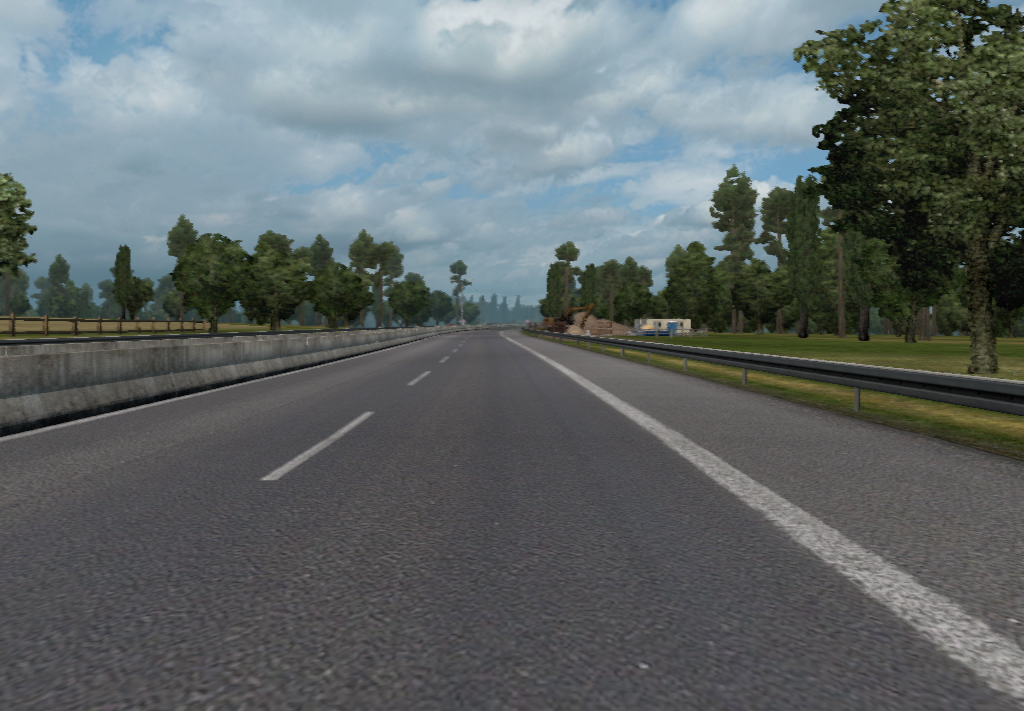
\includegraphics[width=12cm]{img/input.png}
  \caption{Przykładowy obraz wejściowy algorytmu detekcji pasa ruchu}
  \label{fig:inputimg}
  % https://pl.wikipedia.org/wiki/Tesla_Model_S#/media/Plik:2014_Tesla_Motors_Model_S_(rear_view)_Netherlands.jpg
\end{figure}

W najczęstszym przypadku obrazem wejściowym do algorytmu jest obraz z kamery umieszczonej pod pewnym kątem do nawierzchni zamontowanej w okolicy przedniego zderzaka lub atrapy chłodnicy. W niniejszej pracy, większość przetwarzanych obrazów pochodzi z symulatora Euro Truck Simulator 2, gry komputerowej, która posiada zaawansowaną grafikę, która przypomina otaczającą rzeczywistość, a także udostępnia możliwości programistyczne, które ułatwią stworzenie aplikacji do testowania algorytmów wizyjnych co jest założeniem niniejszej pracy. W niniejszej sekcji zostanie opisany algorytm z artykułu \cite{T3}
Autor korzysta w nim z podstawowych operacji przetwarzania obrazów. 



\begin{figure}
  \centering
  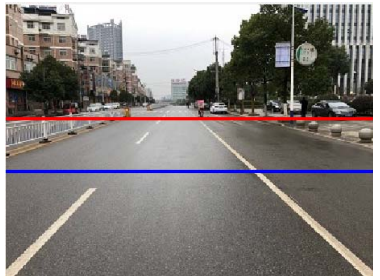
\includegraphics[width=10cm]{img/roi.png}
  \caption{Linie obrazujące granice obszaru poddawanego analizie\cite{T3}}
  \label{fig:roi}
  % artykuł
\end{figure}
Pierwszym krokiem jest wyodrębnienie z obrazu ROI \footnote{ROI (ang.) - Region of interest - obszar obrazu poddawany analizie i dalszemu przetwarzaniu}. Ma to na celu ograniczenie ilości danych poddawanych analizie, a co bardziej istotne odrzuca te fragmenty obrazu, na których na pewno nie będzie jezdni (powyżej czerwonej linii), a także te gdzie obraz linii mógłby być zakłócony. Warto zauważyć, że pomiędzy liniami - czerwoną i niebieską znajduje się prawie dwa razy więcej długości drogi niż w obszarze pod niebieską linią.

Kolejnym etapem jest ekstrakcja pasów ruchu. W większości krajów mają one kolor biały, rzadziej żółty. Są to kolory, które na drodze można rzadko zauważyć w innej funkcji niż malowanie znaków poziomych, w tym linii. Mając na wejściu obraz RGB\footnote{RGB - obraz o trzech składowych barwnych czerwonej(R), zielonej(G) i niebieskiej(B)} można zauważyć, że składowe czerwona i zielona mają większe wartości tam gdzie na obrazie są linie w porównaniu do standardowej nawierzchni jezdni. W artykule, który opisuje ta sekcja zaproponowano następującą metodę segmentacji linii:
\begin{equation}
\label{eq:IMij}
IM(i,j)=\left\{\begin{matrix}
255, & \begin{matrix}
R(i,j)\geq (0.2R_{min}+0.8R_{max})\\ 
G(i,j)\geq (0.2G_{min}+0.8G_{max})
\end{matrix}\\ 
0, & wpp\footnote{w przeciwnym przypadku}.
\end{matrix}\right.
\end{equation}

\begin{equation}
\label{eq:Gij}
G(i,j)=\left\{\begin{matrix}
255, & \begin{matrix}
R(i,j)\geq G(i,j) \geq B(i,j)\\ 
IM(i,j)>0
\end{matrix}\\ 
0, & wpp.
\end{matrix}\right.
\end{equation}

\begin{equation}
\label{eq:Gray}
Gray(i,j)=R(i,j)+G(i,j)-2B(i,j)+0.3*8|R(i,j)+G(i,j)|
\end{equation}

\begin{equation}
\label{eq:GMij}
GM(i,j)=\left\{\begin{matrix}
128, &  Gray(i,j)\geq 0.8*Gray_{m} \\ 
255, & \begin{matrix}
2*Gray_{avg} \leq Gray(i, j) \leq Gray_{m}\\albo\\ 
G(i,j)=255
\end{matrix} \\ 
0,   & wpp.
\end{matrix}\right.
\end{equation}

W równaniu \eqref{eq:IMij} \ ${IM(i,j)}$ oznacza tymczasową macierz cech koloru. ${R(i,j)}$ oznacza jasnośc składowej czerwonej, a ${G(i,j)}$ składową zieloną. ${R_{max}}$, ${R_{min}}$, ${G_{max}}$, ${G_{min}}$ reprezentują maksymalną i minimalną wartość składowej czerwonej, a także maksymalną i minimalną wartość składowej zielonej. W równaniu \eqref{eq:Gray} \ $ Gray(i,j)$ wskazuje na obraz wejściowy w skali szarości, na wartości którego ma wpływ każda ze składowych barwnych. W ostatnim równaniu \eqref{eq:GMij} \ $GM(i,j)$ oznacza obraz wynikowy, na którym zaznaczone jest wysegmentowane poziome oznaczenie jezdni. $Gray_{avg}$ to średnia wartość obrazu w skali szarości w danym wierszu, natomiast $Gray_{m}(i,j)$ oznacza wartość maksymalną dla danego wiersza.

\begin{figure}
  \centering
  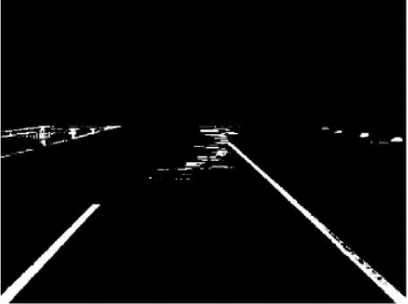
\includegraphics[width=7cm]{img/segmentacja.png}
  \caption{Obraz $GM$ -- wysegmentowane linie\cite{T3}}
  \label{fig:segmented}
  % https://pl.wikipedia.org/wiki/Tesla_Model_S#/media/Plik:2014_Tesla_Motors_Model_S_(rear_view)_Netherlands.jpg
\end{figure}


Kolejnym etapem opisywanego algorytmu jest wykrywanie krawędzi, tu zrealizowane za pomocą filtru Canny'ego. Jest to filtr nieliniowy z histerezą. Dobrze sprawdza się do wykrywania krawędzi na obrazach niejednorodnych i rozmytych. Następnie podejmowana jest ekstrakcja cech linii. Na potrzeby wyjaśnienia działania podanego fragmentu algorytmu przyjęto:
\begin{itemize}
\item $IME$ -- Obraz z równania \eqref{eq:GMij} po filtracji filtrem Canny'ego
\item $IMC$ -- Obraz $GM$ z równania \eqref{eq:GMij}
\end{itemize}

Dla każdego piksela w obrazie $IME$ który został oznaczony jako krawędź zostaje sprawdzana następująca zależność:
\begin{equation}
	\begin{matrix}
	IMC(i,j+1)+IMC(i,j)+IMC(i,j-1)+IMC(i-1,j+1)\\
	+IMC(i-1,j)+IMC(i-1,j-1)+IMC(i+1,j+1)+IMC(i+1,j-1)>0
	\end{matrix}
\end{equation}
Jeśli jest ona spełniona, wybrany punkt na obrazie $IME$ zostaje uznany jako krawędź pasa jezdni.

\begin{figure}
  \centering
  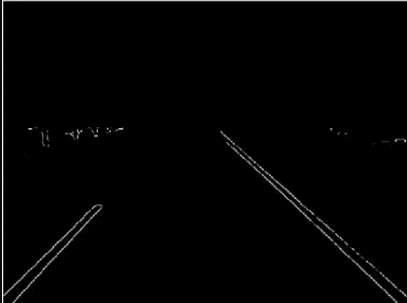
\includegraphics[width=7cm]{img/canny.png}
  \caption{Obraz po zastosowaniu filtra Canny'ego oraz ekstrakcji cech linii\cite{T3}}
  \label{fig:canny}
  % https://pl.wikipedia.org/wiki/Tesla_Model_S#/media/Plik:2014_Tesla_Motors_Model_S_(rear_view)_Netherlands.jpg
\end{figure}

Do ostatecznego wykrycia linii prostych należy użyć zmodyfikowanej transfomaty Hougha( \textit{constraint Hough transform}). Główna różnica pomiędzy nią, a klasyczną transformatą Hougha polega na tym, że wartości $\rho$ i $\theta$ są skwantowane i pogrupowane. Dzięki takiej modyfikacji linie które leżą blisko siebie lub w przypadku nieidalnie prostej linii redukuje się prawdopodobieństwo wielokrotnej detekcji prostej.

\begin{figure}
  \centering
  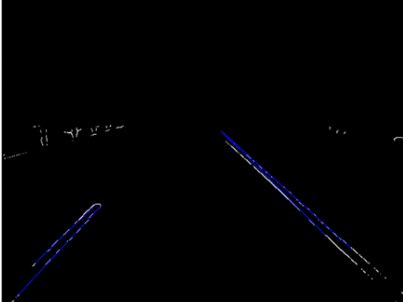
\includegraphics[width=7cm]{img/prehough.png}
  \caption{Wynik algorytmu detekcji linii\cite{T3}}
  \label{fig:result}
  % https://pl.wikipedia.org/wiki/Tesla_Model_S#/media/Plik:2014_Tesla_Motors_Model_S_(rear_view)_Netherlands.jpg
\end{figure}

\subsection{Detekcja zakrętów}
Podobnym zadaniem jest detekcja pasa ruchu w zakręcie. Kształt zakrzywionej linii może być opisany za pomocą paraboli z równania \ref{eq:ld_1}. Zauważono, że fragment drogi bliżej samochodu z reguły jest prosty, zakrzywienie widać powyżej pewnej odległości, a na obrazie powyżej pewnej wysokości. Równanie \ref{eq:ld2} pokazuje model pasa ruchu, gdzie $y_m$ to współrzędna punktu, w którym prosta przechodzi w krzywą.
\begin{equation}
x=a+by+cy^{2}
\end{equation}

\begin{equation}
x=\begin{cases}
a+by,\qquad\qquad y\leq y_{m}\\ c+dy+ey^{2},\qquad y > y_{m} \end{cases}
\end{equation}

gdzie ponadto:
\begin{itemize}
\item $a,b$ -- parametry linii
\item $c,d,e$ -- parametry krzywej
\end{itemize}

Linie prosta i krzywa powinny spotykać się w jedym punkcie, którego współrzędna wysokościowa jest równa $y_m$. Po pewnych przekształceniach otrzymano równanie \ref{eq:ld_3} i \ref{eq:ld_4}.

\begin{equation}
a+by_{m}=c+dy_{m}+ey_{m}^{2}
\end{equation}

\begin{equation}
b = d+2ey_m
\end{equation}

Ostatecznie uzyskano zależność \ref{eq:ld_5} pomiędzy parametrami krzywych.

\begin{equation}
\begin{cases} c=a+\frac{y_{m}}{2}(b-d) \\
e=\frac{1}{2y_{m}}(b-d) \end{cases}
\end{equation}


\section{Detekcja znaków drogowych}

Innym w swojej naturze zadaniem stawianym przed systemami wizyjnymi w pojazdach autonomicznych jest detekcja znaków drogowych. Systemy tego typu pojawiały się dość wcześnie w samochodach pełniąc jedynie funkcję ostrzegawczo-informacyjną. Coraz bardziej dynamicznie rozwijające się systemy wspomagające kierowcę wymagają od subsystemu odpowiedzialnego za detekcję znaków drogowych dużej skuteczności, ponieważ na ich detekcjach opierają decyzje o sterowaniu pojazdem. Istotnym problemem jest brak ujednoliconego zestawu znaków dla całego świata. Obecnie każdy kraj posiada swój zestaw znaków, które w ogólności są podobne, jednak różnice w szczegółach sprawiają problemy systemom wizyjnym. Proponowanym rozwiązaniem jest zbudowanie odpowiednio dużej bazy wzorców znaków i stosowanie określonego zestawu w zależności od lokalizacji. 

Rozwiązanie proponowane w \cite{T2} składa się z dwóch etapów. Pierwszy to detekcja znaku, a drugi to jego klasyfikacja. Do wykrycia znaku drogowego na obrazie pochodzącym z kamery umieszczonej w samochodzie użyto \textit{Radial Symmetry Transform} do detekcji znaków ograniczenia prędkości. Obecnie stowane metody detekcji bazują na segmentacji koloru lub kształtu. 

\subsection{Radial Symmetry Transform}
Klasyczne detektory kształtu wymagają często zamkniętych konturów. Odporne techniki takie jak transformata Hougha dla kół wymaga dużych nakładów obliczeniowych dla dużych obrazów. \textit{Fast radial symmetry detector - (ang. Szybki radialny detektor symetrii)} może być używany jako detektor w czasie rzeczywistym. Znakomita większość znaków z ograniczeniem prędkości to koło z czerwonym brzegiem i wartością ograniczenia w środku na białym tle. Opisywana metoda detekcji jest kompatybilna ze wszystkimi głównymi metodami klasyfikacji takimi jak np. SVM (ang. Support Vector Machine - maszyna wektorów wspierających). Główną zaletą użycia opisywanej metody jest fakt, że wraz z informacją o wykrytym znaku podawana jest skala znaku, co znacząco ułatwia klasyfikację, ponieważ niepotrzebne staje się używanie szablonów o wielu rozmiarach dla wielu różnych rozdzielczości.

Szybki radialny detektor symetrii jest wariantem transformaty Hougha dla wyszukiwania okręgów. Jest on wykonywany w porządku $kp$, gdzie $k$ oznacza liczbę promieni, które są szukane, a $p$ liczbę pikseli. Stanowi to różnicę w stosunku do klasycznej transformaty Hougha wykonywanej w porządku $kbp$, gdzie każdy piksel na obrazie krawędzi ,,głosuje'' dla każdego koła z dyskretnego zestawu promieni. $b$ oznacza dyskretyzację zestawu promieni okręgów, które mogą przechodzić przez aktualnie analizowany punkt.

\begin{figure}
  \centering
  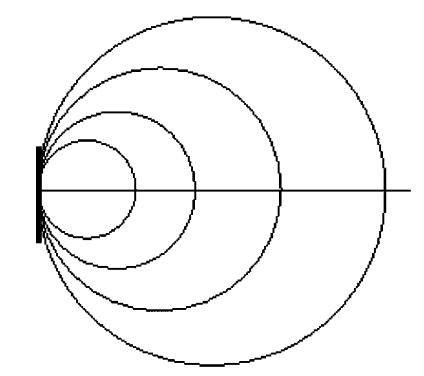
\includegraphics[width=7cm]{img/fsrd1.png}
  \caption{Algorytm głosowania - dla danego punktu krawędzi środki rodziny krawędzi leżą na lini prostopadłej do krawędzi\cite{T2}}
  \label{fig:frsd1}
\end{figure}

FRSD eliminuje czynnik $b$ poprzez pozyzskanie informacji o kierunku gradientu z detektora krawędzi Sobela. Zamiast sprawdzania każdego możliwego kierunku promienia, sprawdzany jest jedynie kierunek prostopadły do kierunku gradientu co jest widoczne na rysunku \ref{fig:frsd1}. Powoduje to, że przestrzeń rozwiązań z trójwymiarowej staje się dwuwymiarowa, co pozwala na używanie algorytmu w czasie rzeczywistym. Operacja radialnej detekcji symetrii może być prosto zrozumiana jako rozważenie wszystkich możliwych okręgów, których dany piksel może być częścią, jeżeli znany jest kierunek krawędzi, to okręgi są szukane tylko na linii prostopadłej do krawędzi (rys. \ref{fig:frsd2}).

\begin{figure}
  \centering
  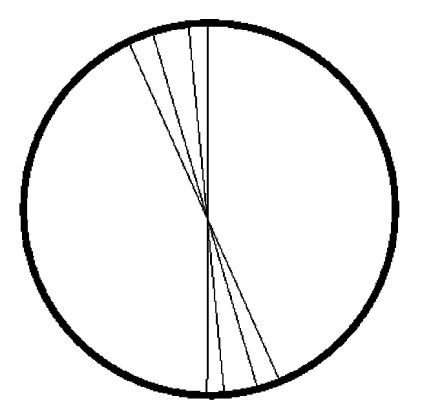
\includegraphics[width=7cm]{img/fsrd2.png}
  \caption{Zachowanie FRSD dla okręgu, zauważalne przecięcie średnic skutkuje istnieniem maksimum lokalnego w środku okręgu.\cite{T2}}
  \label{fig:frsd2}
\end{figure}

Praktyczna realizacja jest wykonywana na obrazie cyfrowym, więc promień jest podzielony na kilka zakresów długości. Istotne jest poprawne dobranie ograniczeń na długość promienia. Na rysunku \ref{fig:tsd} po prawej stronie jest widoczny znak ograniczenia prędkości, który powinien zostać wykryty. Daje się zauważyć, że można dobrać odpowiednie zakresy promienia dla wykrywanych znaków, a także wyodrębnić obszar na którym znaki na pewno nie będą się pojawiać, a także taki, na którym należy wykonać detekcję.
\begin{figure}
  \centering
  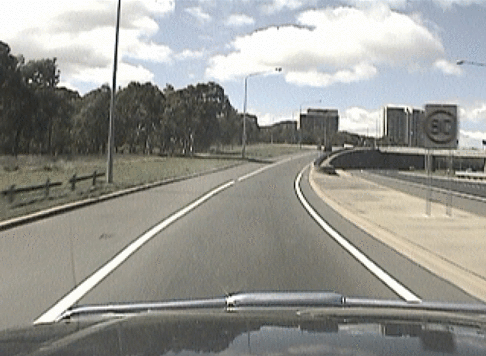
\includegraphics[width=7cm]{img/znaki1.png}
  \caption{Obraz wejściowy algorytmu detekcji znaków drogowych\cite{T2}}
  \label{fig:tsd}
\end{figure}

%\begin{figure}
%\centering
%\subfloat[obraz 1]{\label{fig:znaki2}
%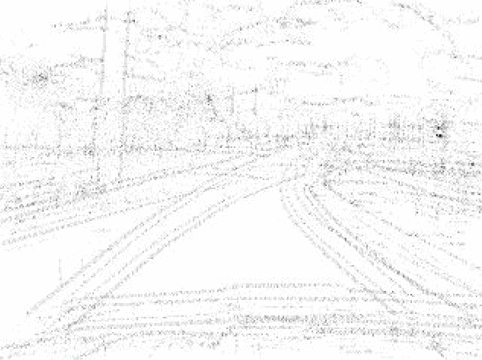
\includegraphics[width=0.3\textwidth]{img/znaki2.png}}
%\quad
%\subfloat[obraz 2]{\label{fig:znaki3}
%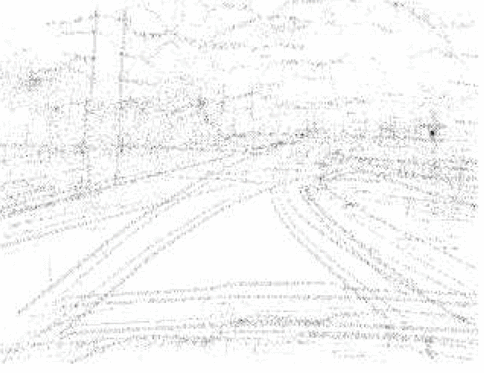
\includegraphics[width=0.3\textwidth]{img/znaki3.png}}
%\caption{Wyniki detekcji, gdy zakres promieni jest zbyt mały \protect\subref{subfigure_a} i zbyt duży, \protect\subref{subfigure_b}.}
%\label{fig:tsd1}
%\end{figure}

\begin{figure}[h]
	\centering
	\begin{subfigure}{0.35\textwidth}
		\centering
		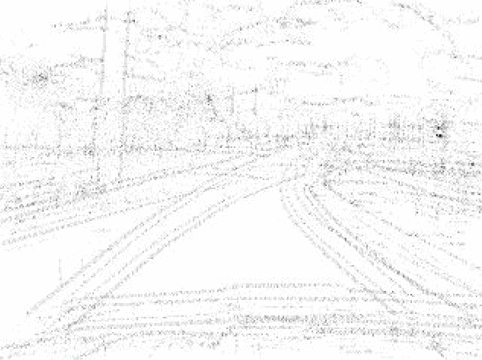
\includegraphics[width=6cm]{img/znaki2.png}
		\subcaption{\label{fig:znaki2}}
	\end{subfigure}
	\begin{subfigure}{0.35\textwidth}
		\centering
		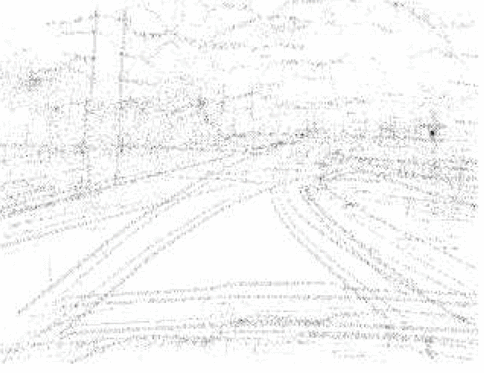
\includegraphics[width=6cm]{img/znaki3.png}
		\subcaption{\label{fig:znaki3}}
	\end{subfigure}
	
	\caption{\label{fig:details}Wyniki detekcji, gdy zakres promieni jest zbyt mały \protect\subref{fig:znaki2} i zbyt duży \protect\subref{fig:znaki3}.\cite{T2}}
\end{figure}

\section{Detekcja świateł drogowych}
\label{sec:tl}
Kolejnym istotnym elementem systemów umieszczanych w pojazdach autonomicznych jest detekcja świateł drogowych. Informują one o możliwości przejazdu przez skrzyżowanie lub rondo i możliwości znalezienia się na trasie kolizyjnej w stosunku do innych użytkowników drogi. Światła drogowe spotykane są głównie w miastach, lecz wraz z rozwojem infrastruktury widywane są w mniejszych miejscowościach. Słupy z zamontowanymi światłami mogą być widoczne na prawej lub lewej krawędzi jezdni, a także nad nią.

\subsection{Detekcja świateł drogowych z użyciem informacji o kolorze i krawędziach}
Światła drogowe na świecie są ustandaryzowane. Istnieją trzy kolory: czerwony, żółty i zielony. Każdy kolor niesie za sobą informację: czerwony - stój, żółty - przygotuj się do zmiany z zielonego na czerwony lub odwrotnie i zielony, który oznacza jedź. Jedyną znaną odchyłką jest odpowiednik światła żółtego w Stanach Zjednoczonych, który jest pomarańczowy.

\begin{figure}
  \centering
  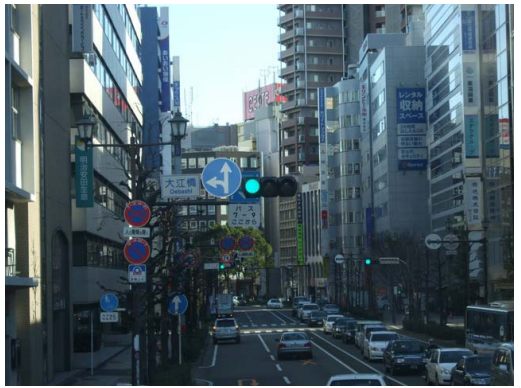
\includegraphics[width=7cm]{img/tl_input.png}
  \caption{Obraz wejściowy algorytmu detekcji świateł drogowych\cite{T4}}
  \label{fig:tl_input}
\end{figure}

Masako Omachi w artykule \cite{T4} proponuje algorytm, który bazuje na informacji o kolorze i krawędzi znajdujących się na obrazie. Światła drogowe mają z góry ustalony kształt - są okrągłe. Istnieją warianty ze strzałkami, lecz opisywany poniżej algorytm służy do detekcji świateł, które w \cite{Kodeks} mają kształ pełnego koła.

Rysunek \ref{fig:tl_input} pokazuje przykład sceny zawierającej światła drogowe. W opisywanej metodzie przestrzeń barw jest konwertowan do znormalizowanej przestrzeni RGB. Normalizacja przestrzeni RGB polega na zmapowaniu wartości pikseli do przedziału $[0,255]$. A także ,,rozsunięciu'' wartości pikseli na obrazie tak, by znajdowały się w całym możliwym zakresie wartości:
\begin{equation}
R=\left\{\begin{matrix}
0, &  s=0\\
\frac{r}{s} & w p.p.
\end{matrix}\right.
\end{equation}
\begin{equation}
G=\left\{\begin{matrix}
0, &  s=0\\
\frac{g}{s} & w p.p.
\end{matrix}\right.
\end{equation}
\begin{equation}
B=\left\{\begin{matrix}
0, &  s=0\\
\frac{b}{s} & w p.p.
\end{matrix}\right.
\end{equation}
gdzie:
\begin{itemize}
\item$r,g,b$ -- składowe czerwona, zielona i niebieska nieznormalizowanego obrazu,
\item$s = r+g+b$
\item$R,G,B$ -- składowe czerowna, zielona i niebieska znormalizowanego obrazu.
\end{itemize}


\begin{figure}
  \centering
  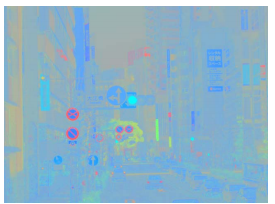
\includegraphics[width=7cm]{img/tl_norm.png}
  \caption{Efekt normalizacji przestrzeni barw\cite{T4}}
  \label{fig:tl_norm}
\end{figure}

Efekt przeniesienia przestrzeni barw do znormalizowanej przestrzeni RGB jest widoczny na rysunku \ref{fig:tl_norm}.
Następnie poprzez progowanie każdej ze składowych uzyskuje się kandydatów do detekcji świateł drogowych. Decyzja o tym czy piksel neleży lub nie do światła drogowego jest podejmowana na podstawie poniższych warunków:
\begin{equation}
R>200 \wedge G< 150 \wedge B<150
\end{equation}
lub
\begin{equation}
R>200 \wedge G> 150 \wedge B<150
\end{equation} 
lub
\begin{equation}
R<150 \wedge G>240 \wedge B>220
\end{equation}.

\begin{figure}
  \centering
  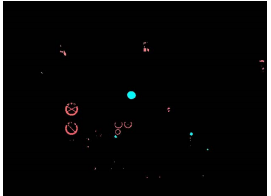
\includegraphics[width=7cm]{img/tl_thresh.png}
  \caption{Rezultat progowania w celu wykrycia obszarów będących kandydatami do bycia światłami drogowymi\cite{T4}}
  \label{fig:tl_thresh}
\end{figure}

Rezultat progowania jest widoczny na rysunku \ref{fig:tl_thresh}. Następnym krokiem jest wykrycie krawędzi na obrazie z kandydatami do detekcji świateł. Jedną z opcji jest użycie filtru Sobela. Ostatnim etapem, jako, że światła drogowe mają jasno określony kształt jest użycie transformaty Hougha dla okręgów, by wykryć właściwe światła drogowe. W artykule stosowana jest zmodyfikowana transformata Hougha do wyszukiwania okręgów, która polega na ustaleniu stałej długości promienia. Klasyczna transformata Hougha jest opisana w sekcji \ref{sec:vision_algs}.

\subsection{Wnioski i rezultaty}
Opisany algorytm detekcji świateł drogowych daje lepsze wyniki niż użycie standardowej przestrzeni barw i klasycznej transformaty Hougha dla okręgów. Porównanie jest zamieszczone w tabeli \ref{tab:tl_results}. Główną zaletą opisywanej metody detekcji świateł drogowych jest fakt, że poprawnie odrzuca ona obrazy znaków drogowych, które również mają okrągłe kształy i jednolite kolory na krawędziach. Algorytm bierze dodatkowo pod uwagę czy kolor na krawędziach jest taki sam jak wewnątrz kształtu, co pozwala skutecznie odrzucić np. znaki zakazu.
Problemem, który napotyka algorytm są tylne światła innych pojazdów, które mają jednolity kolor (z reguły czerwony), a także kształt zbliżony do czerwonego. Przykładowy błąd detekcji jest ukazany na rysunku \ref{fig:tl_err}.

\begin{figure}
  \centering
  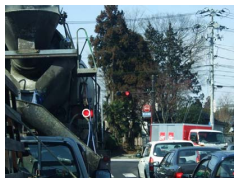
\includegraphics[width=7cm]{img/tl_err.png}
  \caption{Przykład błędnej detekcji tylnego światła traktora\cite{T4}}
  \label{fig:tl_err}
\end{figure}

\begin{table}[]
\centering
\caption{Porównanie klasycznego algorytmu detekcji świateł i opisanego w tej pracy\cite{T4}}
\begin{tabular}{lllll}
\cline{1-3}
\multicolumn{1}{|l|}{}                           & \multicolumn{1}{l|}{Algorytm klasyczny} & \multicolumn{1}{l|}{Algorytm opisany w tym rozdziale} &  &  \\ \cline{1-3}
\multicolumn{1}{|l|}{Dokładność}                 & \multicolumn{1}{l|}{20/30}              & \multicolumn{1}{l|}{26/30}                            &  &  \\ \cline{1-3}
\multicolumn{1}{|l|}{Czas przetwarzania {[}s{]}} & \multicolumn{1}{l|}{0.561}              & \multicolumn{1}{l|}{0.347}                            &  &  \\ \cline{1-3}
                                                 &                                         &                                                       &  & 
\end{tabular}
\label{tab:tl_results}
\end{table}



\section{Detekcja samochodu poprzedzającego}
\label{sec:car_general}
Istotnym zadaniem stawianym przed algorytmami wizyjnymi stosowanymi w pojazdach autonomicznych jest detekcja samochodów w najbliższym otoczeniu pojazdu. Detekcja może być wspierana odczytami z radaru lub lidaru, jednak w poniższej sekcji zostanie opisany algorytm bazujacy jedynie na obrazie z kamer. Większość współczesnych samochodów widzianych od tyłu zachowuje symetrię wględem pionowej osi przechodzącej przez środek pojazdu. 

Pierwszym wstępnym krokiem jest zbadanie możliwych pozycji samochodów na obrazie i oznaczenie ich jako ROI. Dla systemu z fuzją danych wizyjnych i radarowych, może to być zrobione poprzez poprzez analizę odległości i prędkości względnej, czyli danych uzyskanych z radaru. Dla systemu, który posiada jedną kamerę pozycja samochodów musi być wyznaczona tylko na podstawie ruchu samochodów na obrazie w czasie.

Opisywany algorytm korzysta z detektora symetrii, który działa w następujący sposób. Dla każdego piksela wyznaczana jest liczba punktów, która jest wartością bezwzględną z różnicy wartości pikseli, które są równoodległe od ustalonej osi symetrii. Jest to zwykle robione z użyciem pewnego okna o z góry ustalonym rozmiarze dobieranym tak, aby pasować do rozmiaru samochodów, które mogą znajdować się na obrazie. Będąc świadomym faktu, że samochód im jest dalej od kamery, tym jest mniejszy zastosowano kilka predefiniowanych rozmiarów okien. Wartości wskaźnika symterii mogą być obliczne dla każdego punktu na obrazie. Piksele z dużą jego wartością są dobrymi kandydatami do należenia do osi symetrii. Wyliczanie wskaźnika symetrii dla każdego punktu na obrazie jest bardzo czasochłonne, więc zdecydowano się na jego wyznaczanie tylko na wcześniej określonych poziomych liniach, które z grubsza pokrywają obszar, na którym mogą znajdować się samochody. Do obliczania wskaźnika symetrii może być użytych kilka cech obrazu takich jak: wartości pikseli w skali szarości, obraz krawędzi, składowa S w przestrzeni barw HSV. Szukanie obrazu samochodu na obrazie w skali szarości jest szybsze, jednak wrażliwe na na zmiany oświetlenia (noc, deszcz). Dobrze sprawdza się badanie nasycenia w przestrzeni barw HSV, ponieważ uniezależnia to obraz samochodu od ogólnej jasności otoczenia i częściowo od pogody.

\subsection{Przebieg algorytmu bazującego na operatorze symetrii}
Pierwszym krokiem jest wygenerowanie obrazu krawędzi na podstawie obrazu w skali szarości lub składowej S przestrzeni barw HSV. W opisanym algorytmie zaproponowano detektor Canny'ego. Rysunek \ref{fig:car_edge} pokazuje rezultat wykrywania krawędzi dla typowego obrazu zawierającego samochód poprzedający. Opierając się na znanej pozycji kamery i jej pochyleniu względem nawierzchni drogi można określić obszar na obrazie, na którym będą szukane samochody. Poziome ograniczenia znajdują się pomiędzy horyzontem i początkiem widocznej drogi na dole obrazu. Pionowe ograniczenia są ustawione tak, by odpowiadać lewemu i prawemu ograniczeniu jezdni. 

\begin{figure}
  \centering
  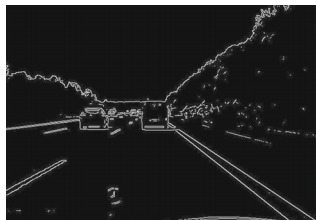
\includegraphics[width=7cm]{img/car_canny.png}
  \caption{Obraz z samochodami po filtracji filtrem Canny'ego\cite{T1}}
  \label{fig:car_edge}
\end{figure}

Jak wspomniano w sekcji \ref{sec:car_general}, w celu zredukowania czasu obliczeń nie każdy piksel w wybranym obszarze jest analizowany. Obliczenia dotyczące symetrii są przeprowadzane tylko dla 15 równoodległych linii skanu (rys. \ref{fig:car_scan_lines1}). Wejściowa rozdzielczość obrazu nie ma znaczenia dla obliczeń. Dzieje się tak ponieważ algorytm wykrywa tylko maksima wzdłuż linii skanu.

\begin{figure}
  \centering
  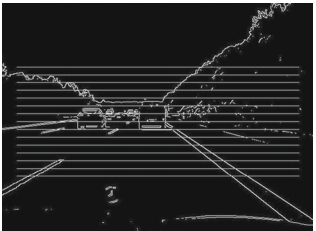
\includegraphics[width=7cm]{img/car_lines.png}
  \caption{Obraz z samochodami po filtracji filtrem Canny'ego i zaznaczonymi liniami skanu\cite{T1}}
  \label{fig:car_scan_lines1}
\end{figure}

Kolejnym krokiem jest detekcja symetrii. Jest ona przeprowadzana dla każdego punktu leżącego na linii skanu. Wartość operatora symetrii dla piksela wyraża się wzorem:

\begin{equation}
SymVal(x,y)=\sum_{x'=1}^{W/2}\sum_{y'=y-H/2}^{y+H/2}S(x, x', y')
\end{equation}
gdzie:
\begin{itemize}
\item
\begin{equation}
S(x,x',y')=\begin{cases}
2 & \text{ gdy } I(x-x',y')=I(x+x',y')=1 \\ 
-1 & \text{ gdy } I(x-x',y')\neq I(x+x',y') \\ 
0 & \text{ w p.p. }
\end{cases}
\end{equation}
\item $W$ -- szerokość okna
\item $H$ -- wysokość okna
\item $I(x,y)$ -- wartość piksela o współrzędnych $x,y$
\end{itemize}

Szerokość okna powinna być właściwie ustawiona, aby poprawnie wykrywać symetryczne obiekty o różnych rozmiarach. W trakcie eksperymentów wykazano, że optymalne wartości $W$ mieszczą się w przedziale $[8,12]$.

\begin{figure}
  \centering
  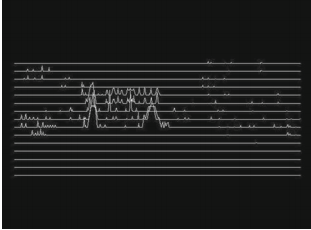
\includegraphics[width=7cm]{img/tl_peaks.png}
  \caption{Wartości wskaźnika symetrii wyznaczone dla linii skanu\cite{T1}}
  \label{fig:car_scan_lines}
\end{figure}

Na rysunku \ref{fig:car_scan_lines} widać, że w niektórych punktach istnieją maksima, które wskazują, że dany punkt może należeć do osi symetrii. Wybiera się maksima i stosuje progowanie, to znaczy wartości maksimów lokalnych poniżej pewnej wartości są odrzucane. Zwykle wartości poniżej określonego progu wskazują na małe, symetryczne elementy tła. Progowania dokonuje się według następującej formuły:
\begin{equation}
SymPts(x,y)=\begin{cases}
1 & \text{ gdy } SymVal(x,y)>T\\ 
0 & \text{ w p.p.}
\end{cases}
\end{equation}

gdzie
\begin{itemize}
\item $T$ - ustalony próg odrzucenia maksimum lokalnego
\end{itemize}


\begin{figure}
  \centering
  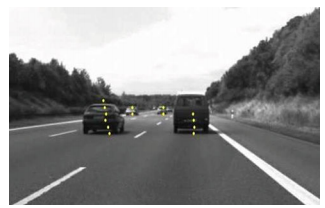
\includegraphics[width=7cm]{img/car_symmetry.png}
  \caption{Wykryte osie symetrii na liniach skanu\cite{T1}}
  \label{fig:car_detected}
\end{figure}

Ostatecznie znalezione maksima oznaczają wykryte osie symetrii względnie dużych obiektów, w tym przypadku samochodów. Widać to na rysunku \ref{fig:car_detected}. Dla każdej linii skanu wykryta oś symetrii jest przesunięta o kilka pikseli, dlatego ostatnim etapem detekcji samochodu jest klasteryzacja.

Uzyskane punkty osi symetrii są klasteryzowane metodą k-średnich. Liczba samochodów na obrazie jest nieznana, więc klasteryzację robi się iteracyjnie, co iterację licząc wariancję, która przy poprawnej liczbie klastrów w stosunku do samochodów na obrazie będzie mniejsza niż określony próg. Końcowy wynik z zaznaczonymi środkami samochodów jest widoczny na rysunku \ref{fig:car_end}

\begin{figure}
  \centering
  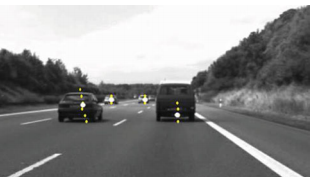
\includegraphics[width=7cm]{img/car_end.png}
  \caption{Wynik algorytmu detekcji samochodów poprzedających\cite{T1}}
  \label{fig:car_end}
\end{figure}

\section{Opis wybranych zagadnień i algorytmów przetwarzania obrazu}
\label{sec:vision_algs}
W tej sekcji zostaną opisane podstawowe algorytmy i zagadanienia dotyczące cyfrowego przetwarzania obrazów, które są używane w zaawansowanych algorytmach wizyjnych w pojazdach autonomicznych.

\subsection{Transformata Hougha dla okręgów}

Systemy wizyjne w pojazdach autonomicznych często mają za zadanie wykrycie obiektów o kształcie koła. Algorytmem do tego przeznaczonym jest transformata Hougha. Istnieje ona w wersji do detekcji prostych i okręgów. Pod pojęciem uogólniona transformata Hougha kryje się algorytm służący do detekcji dowolnego zadanego konturu.

Okrąg można sparametryzować za pomocą następującego wzoru:
\begin{equation}
(x-x_0)^2+(y-y_0)^2=r^2
\end{equation}
gdzie
\begin{itemize}
\item $x_0, y_0$ -- współrzędne środka okręgu
\item $r$ -- promień okręgu
\end{itemize}

\begin{figure}[h]
\centering
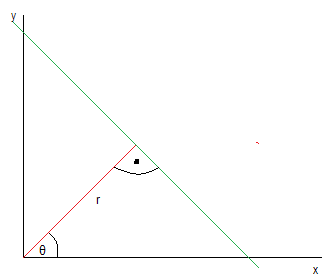
\includegraphics[width=7cm]{img/hough.png}
\caption{Linia w układzie współrzędnych określona za pomocą parametrów $(r, \theta)$}
\label{fig:hough}
\end{figure}

Jeżeli promień będzie ustalony,to okrąg zostanie sparametryzowany za pomocą dwóch liczb. Gdy szukamy okręgów o nieznanych promieniach, rośnie złożoność obliczeniowa, ponieważ wymiar przestrzeni parametrów zwiększa się o jeden.

Możliwa jest również parametryzacja okręgu w biegunowym układzie współrzędnych:
\begin{equation}
x = x_0 + rcos(\theta)
\end{equation}
\begin{equation}
y = y_0 + rsin(\theta)
\end{equation}

po prostym przekształceniu orzymano:

\begin{equation}
x_0 = x - rcos(\theta)
\end{equation}
\begin{equation}
y_0 = y - rsin(\theta)
\end{equation}

Następnie wyznaczana jest przestrzeń Hougha, w której dla każdego piksela obrazu wyznacza się liczbę możliwych okręgów do których mógłby należeć. Wartości maksymalne w przestrzeni Hougha oznaczają wykryty okrąg.

\subsection{Przestrzenie barw}

Podstawową przestrzenią barw jest RGB. Przestawiona na rysunku \ref{fig:rgb} za pomocą sześcianu. Każda składowa jest odpowiedzialna za informację o zawartości danego koloru. Jej zaletą jest prostota opisu, natomiast wadą jest fakt, że po niewielkiej zmianie wartościskłądowych otrzymuje się zupełnie inną barwę. Dodatkowo, co jest ważne w przypadku systemów wizyjnych, niewielka zmiana poziomu jasności powoduje duże wahania składowych R, G, B.

\begin{figure}
  \centering
  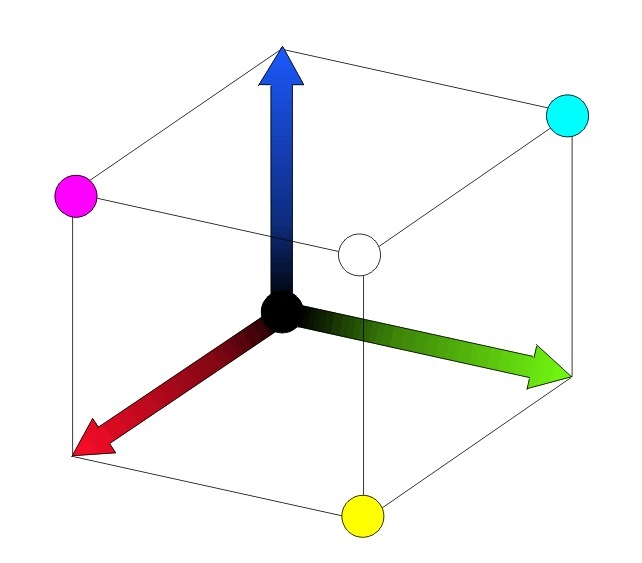
\includegraphics[width=7cm]{img/rgb.jpg}
  \caption{Sześcian przedstawiający przestrzeń barw RGB\cite{W4}}
  \label{fig:rgb}
\end{figure}


\begin{figure}
  \centering
  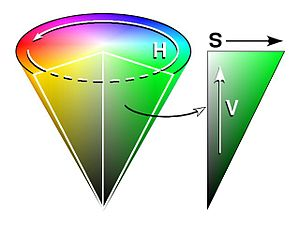
\includegraphics[width=7cm]{img/hsv.jpg}
  \caption{Stożek przedstawiający przestrzeń barw HSV(\textit{źródło: Wikipedia})}
  \label{fig:hsv}
\end{figure}

Drugą, ważną przestrzenią barw używaną w cyfrowym przetwarzaniu obrazów jest przestrzeń HSV. Przedstawiona na rysunku \ref{fig:hsv} za pomocą stożka. Główną zaletą jest to, że przy niewielkich zmianach jasności są bardzo nieduże zmiany w składowej S. Pozwala to na uniezależenienie się w pewnym stopniu od czynników takich jak pora dnia lub pogoda.

\subsection{Filtr Canny'ego}
Podstawowym, dobrze sprawdzającym się detektorem krawędzi jest filtr Canny'ego. Cechuje się właściwościami:

\begin{itemize}
\item niska liczba fałszywych detekcji krawędzi,
\item poprawne wskazywanie pozycji krawędzi. Pozycja krawędzi wskazywana przez detektor powinna odpowiadać jej prawdziwemu położeniu
\item jedna wykryta krawędź przypadająca na rzeczywistą krawędź
\end{itemize}

Detektor krawędzi Canny'ego jest algorytmem wieloetapowym:
\begin{enumerate}
\item Usunięcie z obrazu jakichkolwiek szumów. Używany jest filtr Gaussa. Przykładowa macierz filtru pokazana jest na rysunku \ref{fig:canny_gauss}
\begin{figure}[h]
\centering
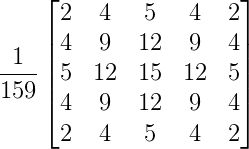
\includegraphics[scale=0.8]{img/canny_gauss.png}
\caption{Maska filtru Gaussa stosowana w wykrywaniu krawędzi}
\label{fig:canny_gauss}
\end{figure}
\item Wyszukiwanie krawędzi z użyciem filtru Sobela o poziomej i pionowej orientacji
\item Określenie wartości gradientu i jego kierunku:

\begin{equation}
G=\sqrt{G_x^2+G_y^2}
\end{equation}

\begin{equation}
\theta=arctan(\frac{G_y}{G_x})
\end{equation}
Kierunek jest zaokrąglany do jednego z czterech możliwych kierunków: \ang{0}, \ang{45}, \ang{90}, \ang{135}

\item Wartości gradientu o niemaksymalnych wartościach są usuwane. Ma to na celu usunięcie pikseli, które prawdopodobnie nie są elementem krawędzi. W wyniku tej operacji pozostają tylko cienkie linie jako krawędzie.

\item Filtr Canny'ego jako argumenty otrzymuje dwa progi - górny i dolny:
\begin{itemize}
\item jeżeli wartość gradientu przekracza górny próg, piksel jest zawsze uznawany jako krawędź
\item jeżeli wartość gradientu nie przekracza dolnego progu, piksel nie jest uznawany za krawędź
\item jeżeli wartość gradientu jest pomiędzy dwoma progami, jest krawędzią, tylko wtedy gdy jest połączony z pikselem, który został sklasyfikowany jako krawędź
\end{itemize}
Twórca filtru rekomenduje stosunek progów filtru pomiędzy 2:1 i 3:1
\end{enumerate}
\chapter{Realizacja projektu}
W tym rozdziale zostanie opisana implementacja systemu służącego do testowania algorytmów wizyjnych z użyciem symulatora Euro Truck Simulator 2. Do stworzenia systemu użyto następujących elementów:
\begin{itemize}
\item Python 3.7 - język programowania wysokiego poziomu ogólnego przeznaczenia,
\item gra Euro Truck Simulator 2,
\item SDK (ang. Software Development Kit) udostępnione przez twórców gry,
\end{itemize}
a także bibliotek dołączonych do Pythona:
\begin{itemize}
\item OpenCV 3.1.3 - biblioteka zawierająca funkcje do cyfrowego przetwarzania obrazów,
\item threading - biblioteka wspierająca programowanie wielowątkowe,
\item libWnck - biblioteka zapewniająca komunikację ze środowiskiem graficznym (Window Navigator Construction Kit),
\item uinput - biblioteka pozwalająca symulować kontroler do sterowania grą.
\end{itemize}

System jest opracowany do działania na systemie Ubuntu 18.04 LTS wraz ze środowiskiem graficznym GNOME.

\section{Euro Truck Simulator 2}
Euro Truck Simulator 2 jest to symulator jazdy ciężarówką opracowany przez czeskie studio SCS Software. Pozwala on na jazdę wybranym modelem ciężarówki przez wiele dróg Europy oraz na realizację zleceń na przewóz towarów. Z uwagi na charakter pracy, interesującymi elementami gry jest wysoka jakość grafiki, wiernie odwzorowująca otaczający świat, w tym zestaw znaków i linii drogowych charakterystycznych dla poszczególnych krajów. Kolejnym elementem który opowiada za wyborem tego symulatora jest otwartość na wszelkie modyfikacje. Twórcy gry udostępnili API (ang. application programming interface), a także konsolę, za pomocą której można na bieżąco modyfikować parametry gry takie jak czas, prędkość gry lub pogodę.
Alternatywnym symulatorem, który również był brany pod uwagę jest American Truck Simulator 2, jednak jest on kalką symulatora opisywanego w tej sekcji ze zmienionym obszarem gry z równie dobrą grafiką i wsparciem dla programistów. Kolejną alternatywą są gry z serii Grand Theft Auto, jednak na ich niekorzyść wskazywało gorsze wsparcie dla programistów, a także niewspółmierne zużycie zasobów do uzyskiwanej jakości obrazu (GTA V) lub niskie zużycie zasobów przy niskiej jakości obrazu (GTA: San Andreas). Fakt, że jest to symulator ciężarówki, a nie samochodu osobowego w żaden sposób nie wpływa na podejście do problemu systemów wizyjnych, ponieważ po pierwsze, istnieją aplikacje wspomagające kierowcę samochodu ciężarowego, po drugie jeden z widoków w grze jest umieszczony w miejscu, które znajduje się na wysokości lusterka samochodowego.

Wspomniana konsola dostępna w grze pozwala na błyskawiczną zmianę warunków w symulatorze. Używając następujących komend można zmienić czas, pogodę oraz prędkość gry:

\begin{itemize}
\item g\_ set\_ weather x -- komenda zmieniająca pogodę. Gdy x jest równy 1, pogoda jest deszczowa, natomiast, gdy jest równy 0 pogoda jest słoneczna
\item g\_ set\_ time x -- komenda ustalająca godzinę w grze. W miejsce x należy podać godzinę w formacie hh,
\item warp x -- komenda zmieniająca prędkość gry. W miejsce x należy wpisać współczynnik. Liczba mniejsza od 1 zwolni grę, a większa przyspieszy.
\end{itemize}

\section{Architektura systemu}
Z uwagi na dydaktyczną wartość opisywanego systemu ważnym elementem jest łatwość implementacji systemu analizy obrazu dla przyszłych użytkowników. Z tego powodu zdecydowano się na implementację wieloprocesową, której schemat jest widoczny na rysunku \ref{fig:arch}, w której jeden z procesów jest odpowiedzialny za analizę obrazu i wypracowanie sterowania, a pozostałe za poprawne przechwycenie obrazu z gry i "wstrzyknięcie" wypracowanego sterowania do gry.

\begin{figure}
  \centering
  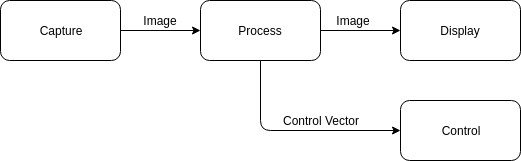
\includegraphics[width=13cm]{img/architektura.png}
  \caption{Schemat architektury aplikacji}
  \label{fig:arch}
\end{figure}

Poszczególne procesy są połączone kolejkami, za pomocą których są transportowane dane pomiędzy nimi. W przypadku tej opisywanej aplikacji w kolejkach umieszczane są obrazy wejściowe i wyjściowe z procesu $Process$, a także wektor sterowań do procesu $Control$. Szybkość działania aplikacji jest zależna od wielu czynników. Głównym elemetem warunkującym jest czas przetwarzania obrazu w bloku $Process$. W zależności od liczby obrazów czekających na przetworzenie w kolejce zmieniany jest interwał pomiędzy poszczególnymi przechwyceniami obrazu w bloku $Capture$. Uniezależnienie przechwytywania obrazu od zapełnienia kolejki spowodowałoby szybkie jej przepełnienie i zabicie aplikacji przez system. Końcowe procesy tj. $Display$ i $Control$ nie wymagajają wyzwalania w zależnosci od czasu przetwarzania obrazu, ponieważ wykonują się bardzo szybko (poniżej 10ms).

Używana biblioteka \textit{multiprocessing}\cite{S2} pozwala na tworzenie podprocesów. Korzyść uzyskana z tego tytułu względem korzystania z wątków polega na tym, że program napisany z użyciem tej biblioteki jest w pełni w stanie korzystać z wielu procesorów lub rdzeni komputera.

\subsection{Przechwytywanie obrazu}
\label{sec:mechanism}
Optymalnym rozwiązaniem byłoby przechwytywanie obrazu wprost z pamięci symulatora, lecz niestety póki co nie istnieją metody pozwalające na takie rozwiązanie. W procesie $Capture$ realizowane są dwa podzadania. Pierwsze polega na znalezieniu i aktywowaniu okna symulatora. Ma to na celu zapobiegnięcie przechwycenia obrazu, gdy okno gry jest przysłonięte przez inną aplikację lub zminimalizowane. Następnie, za pomocą biblioteki libwnck odczytanie współrzędnych okna gry (współrzędne górnego rogu, szerokość i wysokość). Dopiero, gdy jest zapewniony poprawny obraz do przechwycenia jest to robione, a obraz w postaci macierzy o wymiarach 1024x768x3 jest wkładany w kolejkę i wysyłany do procesu przetwarzania i analizy obrazu. Jednorazowe przechwycenie okna zajmuje średnio (około 10ms).

\subsection{Przetwarzanie i analiza obrazu}
Jeśli kolejka wejściowa do procesu nie jest pusta, to obraz jest z niej pobierany, a następnie w zależności od wybranego algorytmu (detekcja linii, detekcja znaków) jest przetwarzany. Poszczególne opisy zaimplementowanych algorytmów znajdują się w sekcjach TODO: numery sekcji z opisem algorytmów. Istotne jest, aby po skończeniu obróbki obrazu i wypracowaniu sterowania włożyć obraz z zaznaczonym wynikiem przetwarzania i wektor sterowań do kolejki.

\subsection{Symulacja kontrolera}
Euro Truck Simulator 2 pozwala użytkownikowi na sterowanie ciężarówką za pomocą licznych kontrolerów. Może to być kawiatura, klawiatura w zestawie z myszką komputerową lub kierownica lub gamepad. W systemach UNIX-owych każde urządzenie wejściowe podpięte do komputera jest widoczne jako plik w lokalizacji $\backslash dev\backslash input\backslash $. Urządzenia generują zdarzenia (ang. eventy), które są przesyłane do korzystających z nich aplikacji. Biblioteka $uinput$ pozwala na zasymulowanie dowolnego kontrolera i sterowanie nim programowo. Na potrzeby opisywanej aplikacji stworzono zasymulowano kontroler, która posiada trzy osie analogowe: kierownica, gej gazu i gej hamulca. Dodatkowo w celu umożliwienia programowej kontroli nad konsolą, kontroler posiada pełen zestaw klawiszy z układu QWERTY. Podczas inicjalizacji aplikacji jest inicjalizowany kontroler, tak, aby przed rozpoczęciem właściwej rozgrywki i przetwarzania obrazu gra wykryła poprawnie urządzenie do sterowania. Klasa $Control$ posiada metodę $emit$, która odpowiada za wygenerowanie zdarzenia z odpowiednimi wartościami sterowania. Podczas wykonywania tej metody jest sprawdzane czy okno z grą jest aktywne, ponieważ w przypadku wyemitowania sterowania przy nieaktywnym oknie, sterowanie nie będzie poprawnie zintepretowane przez symulator.

\subsection{Wyświetlanie rezultatów}
Wyświetlanie rezultatów jest opcjonalne. Jest realizowane w osobnym procesie ze względu na ustaloną architekturę systemu, która zakłada, że w procesie odpowiedzialnym za przetwarzanie obrazu będzie realizowane tylko przetwarzanie. Wyświetlanie obrazu jest realizowane za pomocą funkcji biblioteki OpenCV $imshow()$.


\section{Opis implementacji algorytmów wizyjnych użytych w symulatorze}
W tej sekcji zostaną opisane algorytmy służące do przetestowania działania frameworku stworzonego w ramach pracy magisterskiej. Cele jakie są postawione przed zaimplementowanym frameworkiem to: przetwarzanie obrazu w czasie rzeczywistym lub do niego zbliżonym, dostęp do wirtualnego kontrolera symulowanego w ramach aplikacji.

\subsection{Algorytm detekcji linii}

W symulatorze Euro Truck Simulator znajdują typy dróg z każdego kraju Europy. Zaczynając od szerokich autostrad, poprzez drogi ekspresowe na wąskich i krętych drogach w Alpach kończąc. Zaimplementowany algorytm jest przeznaczony do detekcji linii na drogach, których krzywizna łuku nie jest duża. Przykładowy obraz wejściowy jest widoczny na rysunku \ref{fig:inputimg}. Pierwszym krokiem jest konwersja przestrzeni barw z RGB do HSV. Wybranie składowej S jako obrazu poddawanego analizie (rys. \ref{fig:alg1_S}) pozwala uniezależnić się od pory dnia i pogody.

\begin{figure}
  \centering
  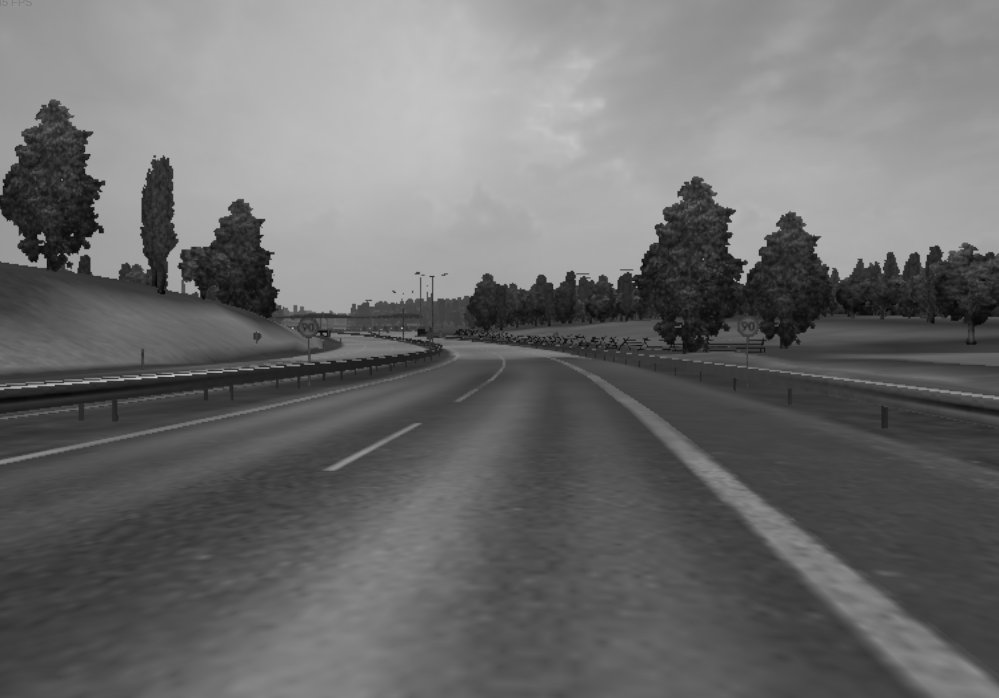
\includegraphics[width=13cm]{img/alg1_gray.jpg}
  \caption{Obraz wejściowy (składowa S)}
  \label{fig:alg1_S}
\end{figure}

Założenie, że obszar jezdni może znajdować się tylko na pewnym obszarze obrazu pozwala zaoszczędzić czas obliczeń. Po wybraniu ROI orzymano obraz \ref{fig:alg1_roi}.

\begin{figure}[h]
	\centering
	\begin{subfigure}{0.35\textwidth}
		\centering
		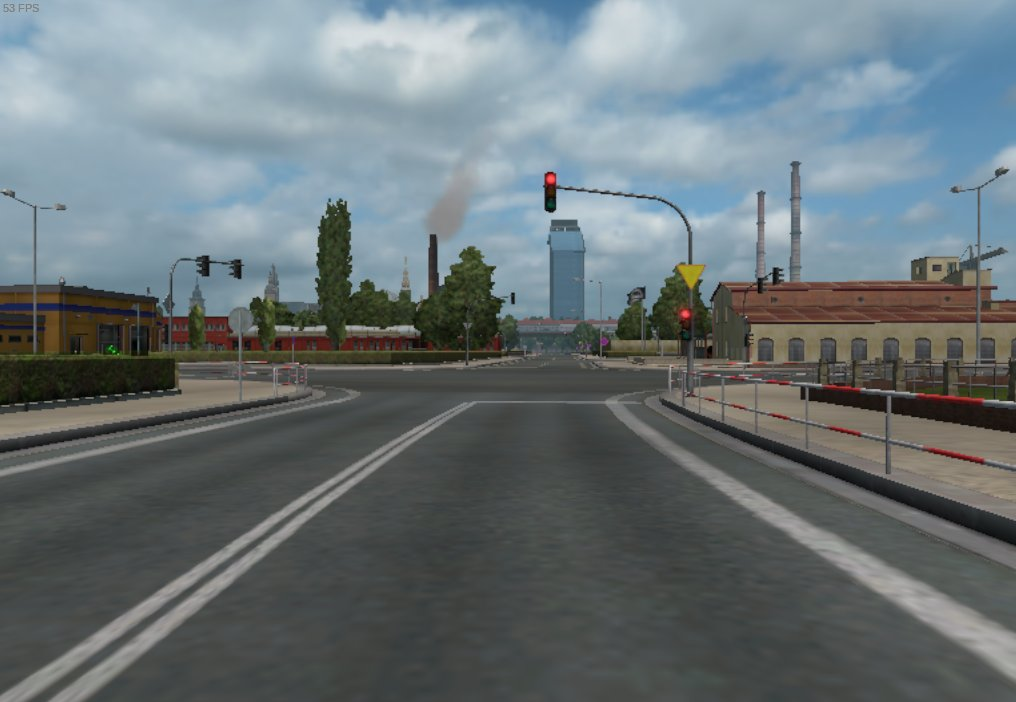
\includegraphics[width=6cm]{img/low_details.jpg}
		\subcaption{\label{fig:low_details}}
	\end{subfigure}
	\begin{subfigure}{0.35\textwidth}
		\centering
		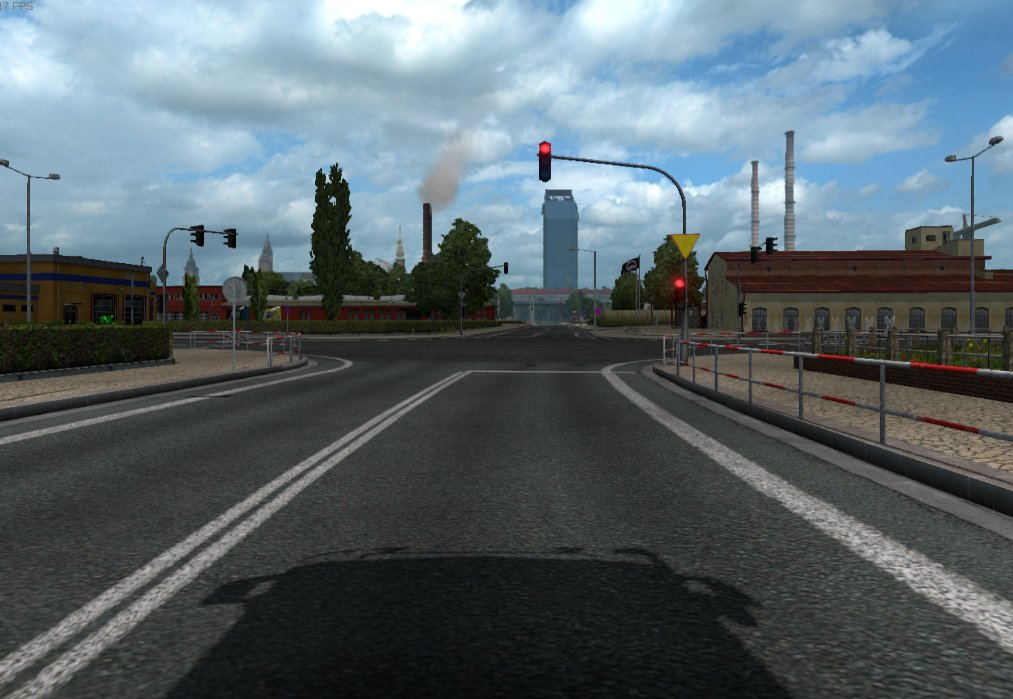
\includegraphics[width=6cm]{img/high_details.jpg}
		\subcaption{\label{fig:high_details}}
	\end{subfigure}
	
	\caption{\label{fig:details1}Porównanie niskich \protect\subref{fig:low_details} i wysokich \protect\subref{fig:high_details} ustawień grafiki symulatora}
\end{figure}

Kolejnym krokiem jest wykrycie krawędzi z użyciem filtru Canny'ego. Progi dobrane są ekperymentalnie. Należy zwrócić uwagę, że gra pozwala na ustalenie jakości grafiki. W związku z tym, każdorazowo po zmianie ustawień należy dobrać współczynniki filtru na nowo. Wraz ze wzrostem jakości grafiki poprawia się jej ostrość. Porównanie niskich i wysokich ustawień graficznych jest widoczne na rysunku \ref{fig:details1}. Kolejną rzeczą wartą uwagi przy wyborze ustawień grafiki jest to, że zarówno praca zaimplementowana w tej pracy jak i gra są uruchamiane na jednej maszynie. W związku z tym wybranie niskich ustawień grafiki pozwoli na przekazanie zasobów obliczeniowych do aplikacji.

\begin{figure}
  \centering
  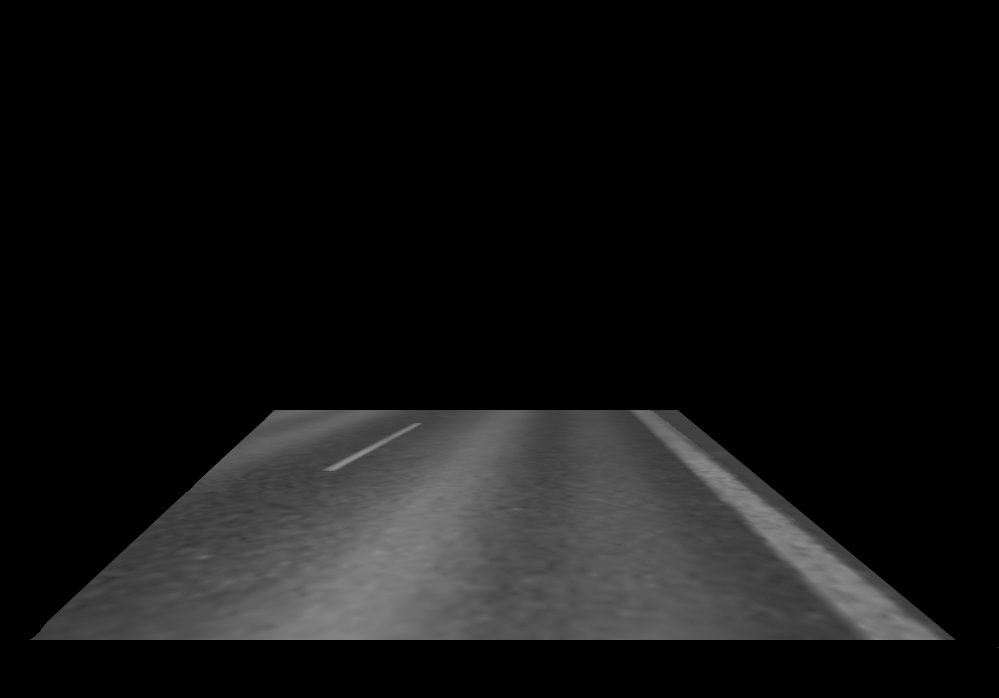
\includegraphics[width=13cm]{img/alg1_roi.jpg}
  \caption{Wyznaczone ROI, na którym można spodziewać się linii}
  \label{fig:alg1_roi}
\end{figure}

Na obrazie krawędzi, za pomocą transformaty Hougha dokonuje się detekcji linii prostych. Linie fałszywe (linie nie będące liniami na jezdni) można odrzucić badając ich parametr $\theta$. Właściwe linie będą pochylone pod odpowienim kątem. Dla opisywanego przypadku właściwym zakresem kąta nachylenia linii jest $\theta < 1.3rad$ dla linii po lewej i $\theta > 2rad$ dla krawędzi prawej.

W celu zaoszczędzenia czasu obliczeń i poprawienia sprawności algorytmu założono, że rezultatem powinna być linia dla każdej z krawędzi jezdni. Jeśli wykryto kilka linii, których parametry są zbliżone, dalszej analizie poddawana jest tylko jedna z nich (rys. \ref{fig:alg1_res}).

Aby wygenerować sterowanie bada się punkt przecięcia wykrytych linii (biały okrąg na rys. \ref{fig:alg1_res}). Zakładając, że kamera jest ustawiona w osi ciężarówki można przyjąć, że każde odchylenie punktu przecięcia wykrytych linii powinno implikować ruch kierownicą.

\begin{figure}
  \centering
  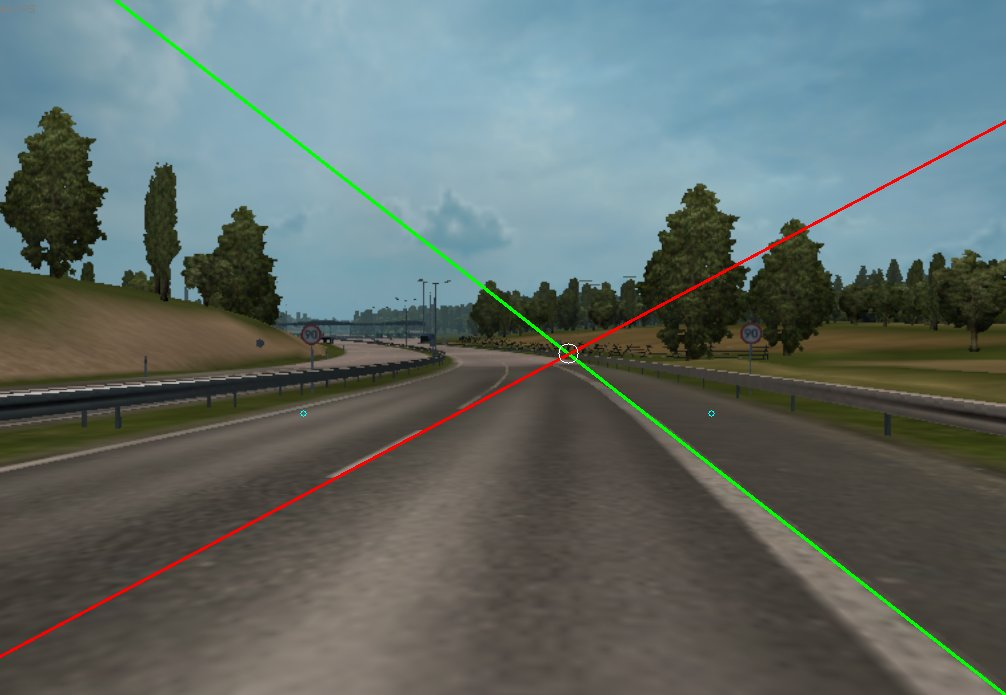
\includegraphics[width=13cm]{img/alg1_res.jpg}
  \caption{Rezultat działania algorytmu}
  \label{fig:alg1_res}
\end{figure}

Średni czas obliczeń potrzebny do przetworzenia jednej klatki wyniósł 59ms, co daje możliwość przetworzenia 17 klatek na sekundę. Jest to wydajność wystarczająca, aby zapewnić stabilność całości algorytmu, ponieważ ciężarówka była w stanie utrzymać się przy stałej prędkości na pasie ruchu długim na ok. 500m.

\subsection{Sytuacje potencjalnie problematyczne}
Jak wspomniano w sekcji \ref{sec:lane_detection} wymagane jest poprawne działanie algorytmu przy zmiennych warunkach oświetlenia i pogody. Symulator oferuje możliwość zmiany tych parametrów poprzez konsolę. Algorytm wykazał skuteczność zarówno przy zmianie godziny gry na późniejszą oraz dodaniu deszczu (rys. \ref{fig:alg1_late} i rys. \ref{fig:alg1_rain})

\begin{figure}
  \centering
  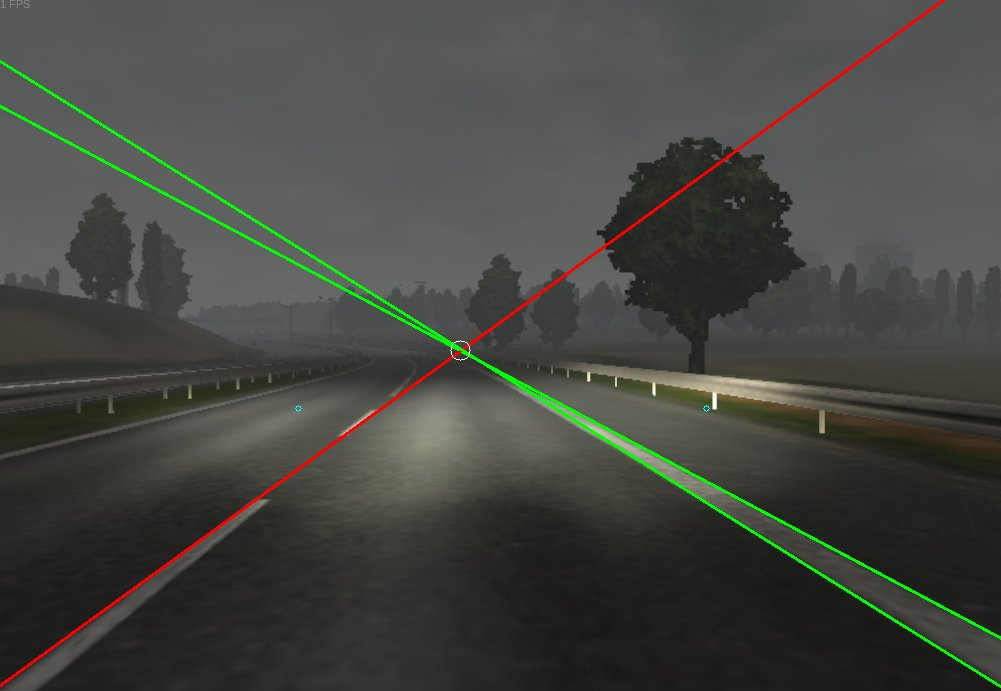
\includegraphics[width=13cm]{img/alg1_late.jpg}
  \caption{Działanie algorytmu podczas trudnych warunków oświetleniowych}
  \label{fig:alg1_late}
\end{figure}

\begin{figure}
  \centering
  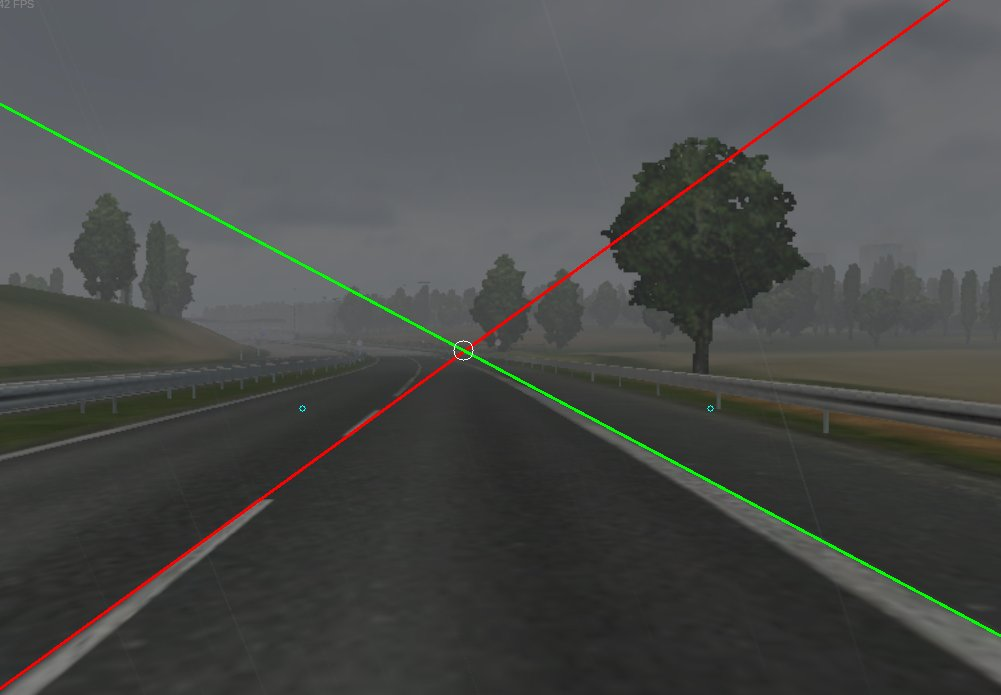
\includegraphics[width=13cm]{img/alg1_rain.jpg}
  \caption{Działanie algorytmu podczas deszczu}
  \label{fig:alg1_rain}
\end{figure}

\subsection{Algorytm detekcji czerwonych świateł drogowych}

Kolejnym algorytmem testowym, który został zaimplementowany w ramach pracy jest uproszczona wersja algorytmu opisanego w sekcji \ref{sec:tl}. Przykładowy obraz wejściowy znajduje się na rysunku \ref{fig:alg2_input}. Dają się tam zauważyć dwa sygnalizatory świetlne, a także kilka znaków drogowych. Sceneria została dobrana tak, aby jednocześnie sprawdzić odporność algorytmu na znaki zawierające czerwoną barwę.

Pierwszym krokiem opisywanej metody jest wyznaczenie kandydatów na światła drogowe. Dobierając ekperymentalnie współczynniki progowania ustalono, że światło czerwone będzie spełniać poniższe warunki:
\begin{equation}
\label{eq:tl}
R>180 \wedge 0 \geq R<100 \wedge B < 120
\end{equation}

gdzie $R, G, B$ oznaczają wartości składowych w przestrzeni RGB.

Aby zapewnić, że inne obiekty spełniające warunek \ref{eq:tl} wykonano operację erozji i dylatacji zwaną również otwarciem morfologicznym. Otrzymany obraz indeksuje się. Iterując po każdym z oznaczonych elementów można sprawdzić jego powierzchnię i proporcje, które muszą spełniać pewne warunki, żeby zostać uznane za światło drogowe.

Aby zmodyfikować algorytm tak, by wykrywał światło zielone lub pomarańczowe należy zmienić wartości progów w warunku \ref{eq:tl}. Do indeksacji kandydatów wykorzystano funkcję biblioteki OpenCV $connectedComponentsWithStats()$, która zwraca listę obiektów wraz z ich statystykami.

\begin{figure}
  \centering
  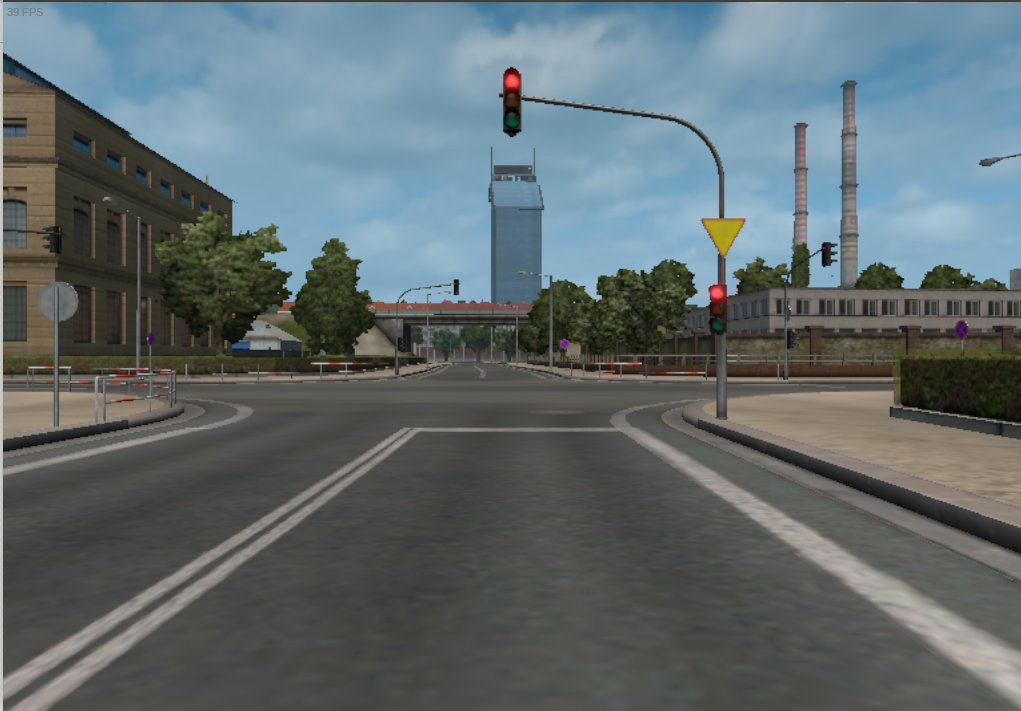
\includegraphics[width=13cm]{img/alg2_input.jpg}
  \caption{Przykładowy obraz wejściowy algorytmu}
  \label{fig:alg2_input}
\end{figure}

\begin{figure}
  \centering
  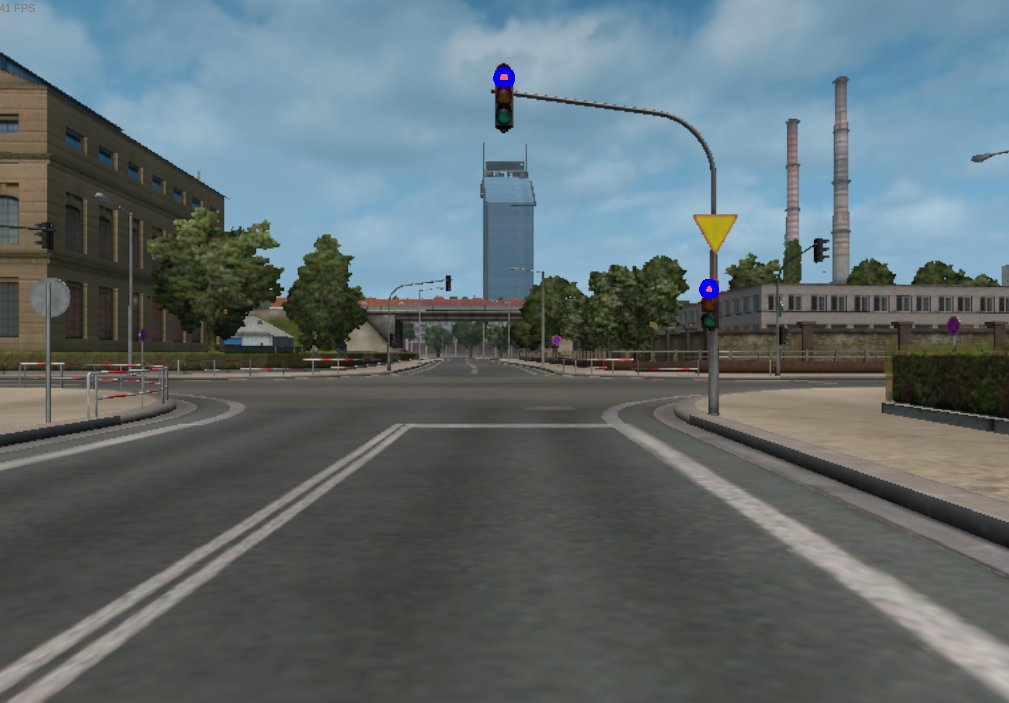
\includegraphics[width=13cm]{img/alg2_res.jpg}
  \caption{Wykryte dwa palące się czerwone światła}
  \label{fig:alg2_res}
\end{figure}

\subsection{Sytuacje potencjalnie problematyczne}
Jak w przypadku każdego z omawianych algorytmów problemem jest zmiana warunków oświetleniowych oraz pogodowych. Nie można jak w przypadku algorytmu detekcji pasa ruchu uniezależnić się od zmian oświetlenia poprzez zastosowanie konwersji do przestrzeni HSV, ponieważ istotną rolę odgrywa tu barwa. Z uwagi na to, że światła drogowe emitują światło, w czasie warunków słabej widoczności i deszczu algorytm poprawnie wykrywał czerwone światło (rys. \ref{fig:alg2_rain} i rys. \ref{fig:alg2_late})

\begin{figure}
  \centering
  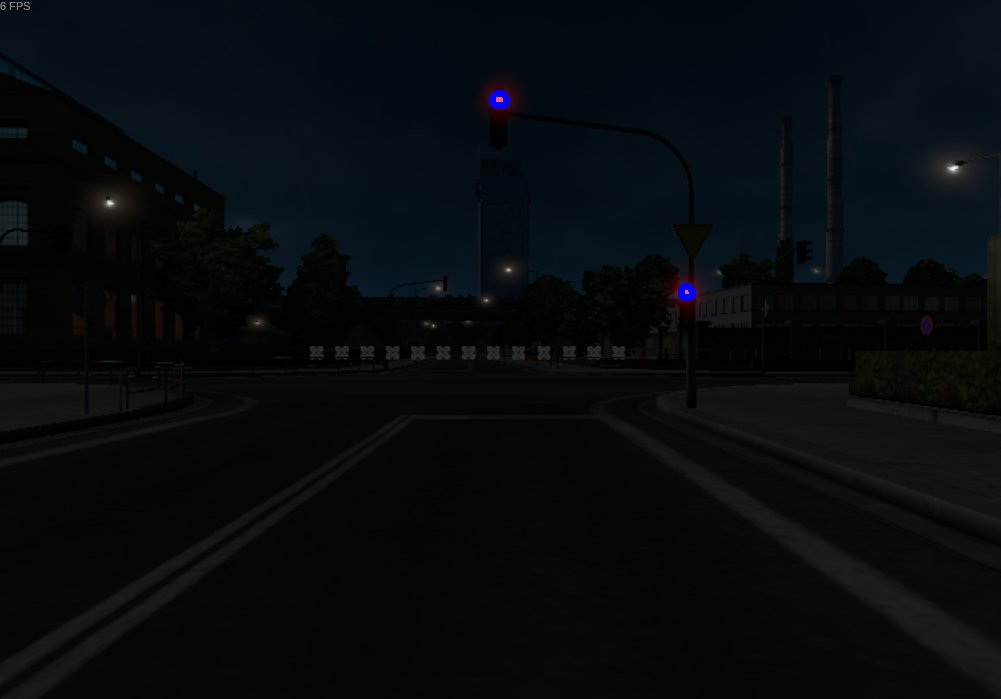
\includegraphics[width=13cm]{img/alg2_late.jpg}
  \caption{Wykryte światła drogowe w warunkach słabego oświetlenia}
  \label{fig:alg2_late}
\end{figure}

\begin{figure}
  \centering
  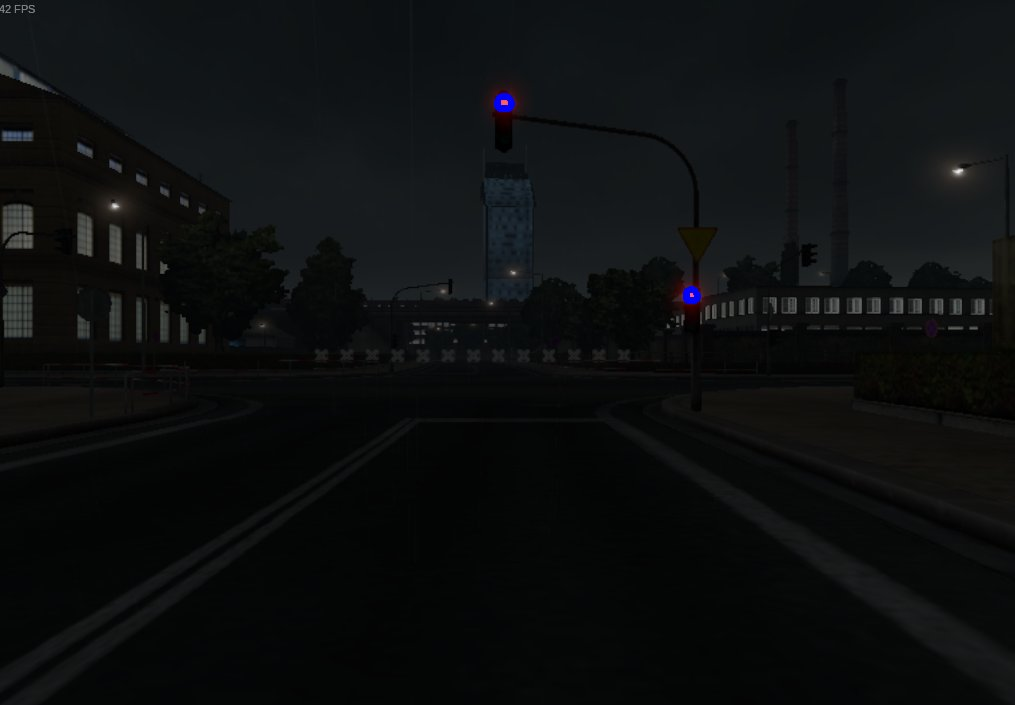
\includegraphics[width=13cm]{img/alg2_rain.jpg}
  \caption{Wykryta sygnalizacja świetlna podczas deszczu}
  \label{fig:alg2_rain}
\end{figure}

\subsection{Detekcja samochodu poprzedającego}
Ostatnim algorytmem, który został zaimplementowany w ramach tej pracy jest detekcja samochodów poprzedających na drodze z użyciem detektora symetrii. Implementacja bazuje na algorytmie opisanym w sekcji \ref{sec:car_general}.

\begin{figure}
  \centering
  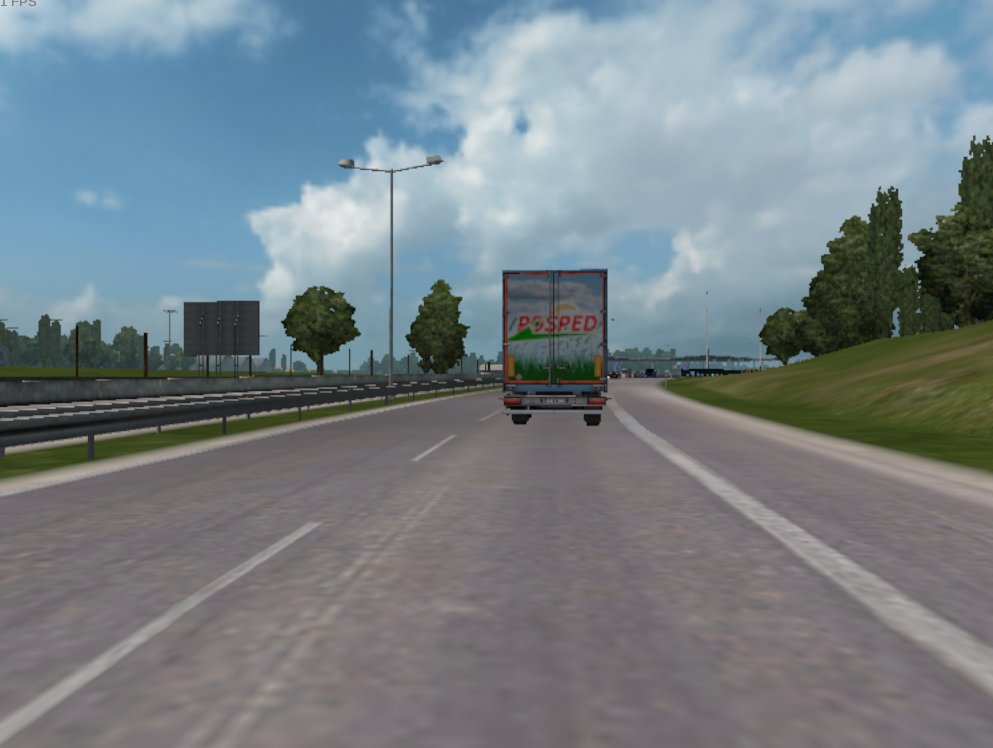
\includegraphics[width=13cm]{img/alg3_input.jpg}
  \caption{Przykładowy obraz wejściowy algorytmu detekcji samochodu poprzedającego}
  \label{fig:alg3_input}
\end{figure}

Zaimplementowany algorytm operuje na obrazach w skali szarości. Przykładowy obraz wejściowy jest pokazany na rysunku \ref{fig:alg3_input}. Daje się na nim zauważyć ciężarówkę poprzedającą samochód. Celem działania algorytmu jest poprawne wykrycie symetrii na tyle naczepy samochodu.

\begin{figure}
  \centering
  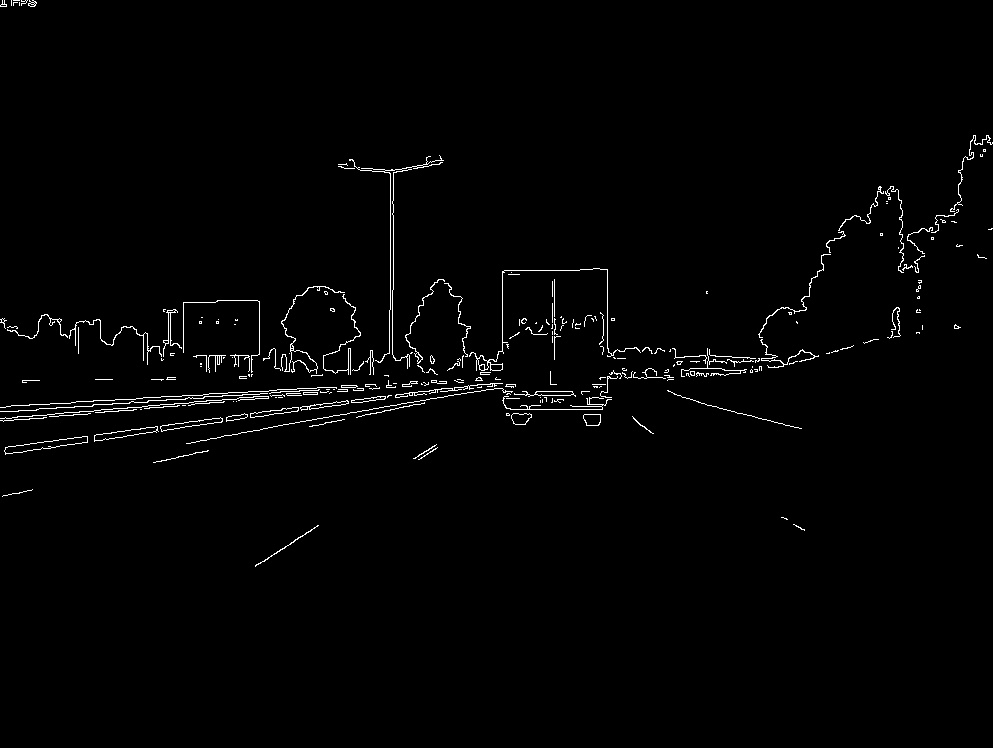
\includegraphics[width=13cm]{img/alg3_canny.jpg}
  \caption{Obraz wejściowy po detekcji krawędzi. Widoczna symetria w układzie krawędzi poprzedającej naczepy}
  \label{fig:alg3_canny}
\end{figure}

Pierwszym krokiem jest filtracja z użyciem filtru Canny'ego. Progi filtru są każdorazowo po zmianie ustawień graficznych symulatora dobierane eksperymentalnie. Efekt filtracji jest widoczny na rysunku \ref{fig:alg3_canny}.

Następnie wyznaczając linie skanu sprawdzana jest symetria obrazów w sposób opisany w sekcji \ref{sec:car_general}. Na każdej z linii skanu wyznaczane są maksima, które wskazują na istnienie osi symetrii. Rezultaty detekcji są umieszczone na rysunkach \ref{fig:alg3_res1} i \ref{fig:alg3_res2}. Daje się zauważyć znaczna liczba detekcji fałszywych. Prawdopodobnie wynika to między innymi z faktu, że w symulatorze obiekty infrastrukrury mają bardziej równomierny i symetryczny kształt.

\begin{figure}
  \centering
  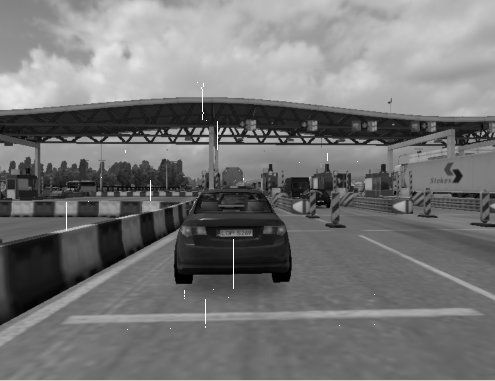
\includegraphics[width=13cm]{img/alg3_res.jpg}
  \caption{Rezultat detekcji samochodu osobowego. Widoczne liczne fałszywe detekcje.}
  \label{fig:alg3_res1}
\end{figure}

\begin{figure}
  \centering
  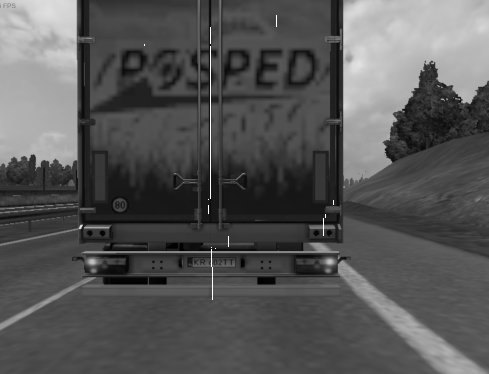
\includegraphics[width=13cm]{img/alg3_res2.jpg}
  \caption{Poprawna detekcja naczepy samochodu ciężarowego}
  \label{fig:alg3_res2}
\end{figure}

Sprawdzono również zachowanie algorytmu w trudnych warunkach pogodowych i słabego oświetlenia. Samochód korzysta ze świateł mijnia, więc najbliższe otoczenie jest dobrze widoczne (rys. \ref{fig:alg3_rain_late}. W tym przypadku również pojawiają się fałszywe detekcje.

\begin{figure}
  \centering
  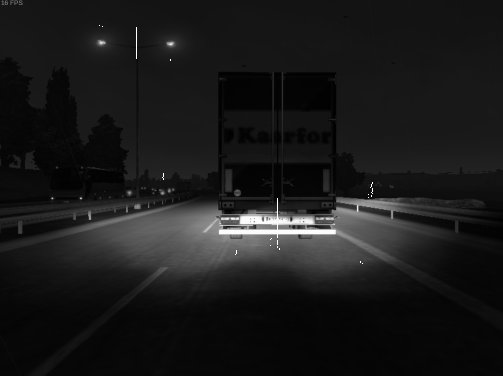
\includegraphics[width=13cm]{img/alg3_res3.jpg}
  \caption{Poprawna detekcja naczepy samochodu ciężarowego w trudnych warunkach oświetleniowych i pogodowych}
  \label{fig:alg3_rain_late}
\end{figure}

Obliczanie wskaźnika symetrii jest operacją bardzo czasochłonną. Średni czas przetworzenia jednej klatki to 5.45 sekundy. Oprócz dużej ilości obliczeń może to być spowodowane mało wydajną implementacją w Pythonie. Implementacja w języku C++ prawdopodobnie przyniosłaby lepsze efekty.

\section{Badania wydajności aplikacji}
Istotną rzeczą jest wydajność całej aplikacji. Powinna ona działać bez widocznych opóźnień, to znaczy, że po przechwyceniu obrazu z symulatora w możliwie najkrótszym czasie powinno zostać wygenerowane sterowanie. Jest to zapewnione poprzez mechanizm opisany w sekcji \ref{sec:mechanism}. Eksperymentalnie dowiedziono, że liczba elementów w kolejkach, zwłaszcza w kolejce pomiędzy modułem $Capture$, a $Process$ nie powinna przekraczać 50. Powyżej tej wartości daje się zauważyć widoczne opóźnienie reakcji systemu sterującego samochodem. Na wykresie przedstawiono rozmiar kolejki w kolejnych iteracjach programu podczas działania systemu wizyjnego odpowiedzialnego za detekcję czerwonego światła.

\begin{figure}
  \centering
  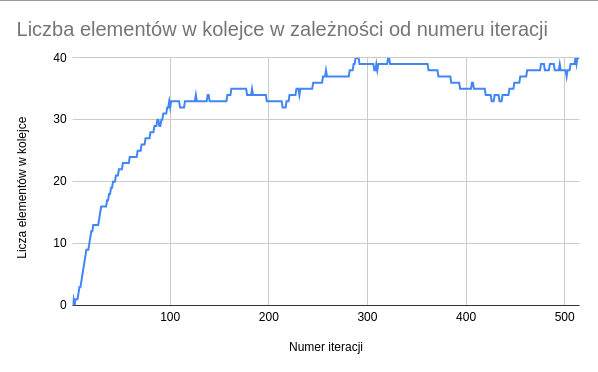
\includegraphics[width=13cm]{img/queue_stats.png}
  \caption{Rozmiar kolejki w trakcie działania programu}
  \label{fig:queue_stats}
\end{figure}

W trakcie implementacji kolejnych systemów wizyjnych używanych w pojazdach autonomicznych należy zwrócić uwagę na optymalizację kodu. Nie powinno się tworzyć wielu kopii obrazu w pamięci, a także z uwagi na asynchroniczny charakter aplikacji nie używać komend typu $wait()$. Ważnym aspektem, który znacząco poprawił wydajność całości systemu było zastosowanie wektoryzacji, czyli wbudowanej w język programowania metody operowania na macierzach. W przypadku, gdy algorytm ze względu na swoją złożoność wykonywałby się zyt długo, należy użyć komendy w konsoli symulatora udostępnionej przez twórców, która zmieni prędkość gry - $warp x$, gdzie $x$ oznacza prędkość (1 - standardowa prędkość rozgrywki).

\section{Ewaluacja systemu}
Celem pracy było stworzenie aplikacji, która będzie w ramach przedmiotu Systemy wizyjne w pojazdach autonomicznych prowadzonego na II stopniu studiów stacjonarnych na kierunku Automatyka i Robotyka pozwalała w przyjazny użytkownikowi sposób na implementację i testowanie algorytmów wizyjnych stosowanych w pojazdach autonomicznych. Przykładowe algorytmy zaimplementowane w ramach tej pracy dowodzą, że jest to możliwe. Korzystanie z aplikacji w ramach zajęć jest zamienną formą w stosunku do korzystania ze zbiorów zdjęć np. KITTI. Nie jest możliwym utworzenie $groundtruth$, aczkolwiek inną formą sprawdzenia czy dany algorytm działa poprawnie jest weryfikacja poprzez zachowanie ciężarówki w symulowanym świecie. Opcjonalne jest generowanie sterowania na podstawie wyników z algorytmów wizyjnych. Końcowy użytkownik może tradycyjnie za pomocą klawiatury lub myszki sterować pojazdem i na bieżąco badać rezultaty osiągane przez algorytm.

Kolejnym etapem rozwoju projektu byłoby stworzenie prostego instalatora, który pobierze i zainstaluje wszystkie potrzebne biblioteki, a także skompiluje zmodyfikowane SDK udostępnione przez twórców. Możliwa jest także dalsza edycja SDK, poprzez umożliwienie odczytu pozostałych zmiennych gry oprócz aktualnej prędkości i stanu pauzy. Pełna lista parametrów jest dostępna w \cite{S3}. Elementem mocno rozbudowującym aplikację byłoby także generowanie danych radarowych na podstawie otoczenia samochodu w symulatorze. Póki co twórcy gry nie udostępniają takiej możliwości przez SDK.


\chapter{Podsumowanie}
Zgodnie z założeniami zrealizowano cele pracy. Dokonano ewaluacji przykładowych algorytmów wizyjnych, które mogłyby znaleźć zastosowanie w pojazdach autonomicznych, a także przetestowano ich działanie z użyciem zaimplementowanego frameworka. Zdaniem autora przygotowany framework nadaje się do użycia w ramach zajęć do testowania algorytmów przetwarzania obrazu. Pozwala w łatwy sposób modyfikować parametry obrazu takie jak natężenie światła, pogodę oraz liczbę otaczających pojazdów. Znaczącą przewagą systemu nad analizą pojedynczych zdjęć jest możliwość przetestowania algorytmów w sytuacjach dynamicznych. Zaimplementowana możliwość sterowania samochodem w symulatorze z pewnością pozwoli na rozbudowanie powstających algorytmów i sprawdzanie ich pod kątem wielu nowych aspektów takich jak np. optymalizacja kodu, by przyspieszyć jego wykonanie.


%\include{rozdzial3}
%\include{rozdzial1}
%\include{rozdzial2}
%\include{tests}



% itd.
 \appendix
 \chapter{Instrukcja do ćwiczenia}

Do prawidłowego działania aplikacji wymagany jest komputer z zainstalowanymi:
\begin{itemize}
\item Python w wersji 3.6 lub wyższej
\item openCV w wersji 3.1.3 lub wyższej
\item system Linux (najlepiej Ubuntu) z systemem okien X11
\item biblioteka multiprocessing języka Python
\item biblioteka Wnck (zapewnia komunikację aplikacji z systemem okien). Instalacja poleceniem: \textsc{apt-get install python3-gi gir1.2-wnck-3.0}
\item biblioteka uinput służąca do symulacji kontrolera (\textsc{https://github.com/tuomasjjrasanen/python-uinput})
\end{itemize}

Ćwiczenie należy zacząć od instalacji symulatora jazdy Euro Truck Simulator 2. Instalacja poprzez platformę Steam jest łatwa i intuicyjna. Dane kont są następujące. Do każdego konta jest przypisana jedna licencja na grę.

Po instalacji należy po raz pierwszy uruchomić grę i ustawić w ustawieniach grafiki wyświetlanie gry w oknie.
Kolejnym krokiem jest odblokowanie konsoli i narzędzi deweloperskich. Aby to zrobić należy zmodyfikować plik \textit{config.cfg}, który powinien znajdować się w lokalizacji: \textit{lsriw/.local/share/Euro Truck Simulator 2/}. Dwie linijki w pliku:
\begin{itemize}
\item \textsc{uset g\_ developer "0"}
\item \textsc{uset g\_ console "0"}
\end{itemize}

należy zmienić na:

\begin{itemize}
\item \textsc{uset g\_ developer "1"}
\item \textsc{uset g\_ console "1"}
\end{itemize}

Aktytowanie tych opcji pozwoli na swobodny dostęp do konsoli w grze oraz używanie narzędzi deweloperskich udostępnionych przez twórców. W przypadku tej aplikacji jest to informacja o prędkości pojazdu oraz stanie gry (pauza/gra).

Następnym etapem jest kompilacja programu, który będzie na bieżąco w trakcie gry zapisywał wspomniane dane do pliku. W folderze z aplikacją znajduje się folder SDK. Tamże należy odnaleźć folder \textit{telemetry} i będąc w nim wykonać polecenie \textsc{make}. Plik wykonywalny \textit{telemetry.so} skopiować do lokalizacji gry: \textsc{/home/lsriw/.steam/steam/steamapps/common/Euro Truck Simulator 2/bin/linux\_ x64/plugins}. Ta operacja sprawi, że gra od tej pory przy każdym uruchomieniu będzie tworzyła plik \textit{telemetry.log}, w którym na bieżąco będzie zapisywana prędkość pojazdu i informacja o aktywnej pauzie. 

Uruchomić symulator, powinno pojawić się okno z informacją o uruchomieniu narzędzi deweloperskich (\ref{fig:appendix1_dev_tools}).

\begin{figure}
  \centering
  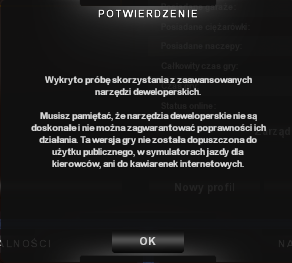
\includegraphics[width=6cm]{img/appendix1_devtools.png}
  \caption{Okno informujące o poprawnym zainstalowaniu SDK}
  \label{fig:appendix1_dev_tools}
\end{figure}

Przy okazji warto przetestować czy konsola również wyświetla się poprawnie. Konsolę aktywuje się klawiszem tyldy.

Ważna uwaga! Zawsze przed uruchomieniem aplikacji należy uruchomić symulator. Przesunięcie okna gry na inny ekran spowoduje niepoprawne działanie aplikacji do testowania algorytmów wizyjnych.

Jeśli wszystkie wymagane biblioteki są zainstalowane, testowo uruchomić aplikację polceniem \textsc{./run.sh}. Aplikacja wymaga dostępu do konta \textit{roota}, ponieważ symulacja kontrolera tego wymaga.

Zaleca się korzystanie w grze z kamery numer 6 (klawisz 6).
W bazowej wersji aplikacji, w której nie są zaimplementowane żadne algorytmy cyfrowego przetwarzania obrazów, obraz przechwycony jest przekazywany do procesu wyświetlającego bez żadnej modyfikacji. W pliku \textit{Process.py} znajduje się funkcja \textsc{process\_ image(self, image)}. Jako argument przyjmuje obraz przechwycony z symulatora. Funkcja zwraca listę złożoną z obrazu przetworzonego oraz wektora sterowania: \textsc{return [image, [None, 0, 0]]}. W tej funkcji należy implementować algorytmy służące do przetwarzania obrazu. Początkowo sugeruje się w ramach testów nie generować sterowania. Dopiero po zapewnieniu pewnej stabilności algorytmu zalecane jest najpierw włączenie kontroli kierownicy samochodu, a następnie programowej kontroli prędkości za pomocą symulowanego pedału gazu i hamulca.

Jak wspomniano, początkowo może być trudne generowanie poprawnego (i sensownego) sterowania. Aby nie programowo nie wpływać na kontroler należy zwracać wektor sterowań w postaci: \textsc{[None, 0, 0]}.

\section{Obsługa kontrolera}
Po zainicjalizowaniu aplikacji gra automatycznie wykryje symulowany kontroler. Posiada on trzy osie analogowe służące do sterowania kierownicą oraz pedałami gazu i hamulca. Analogowa oś kierownicy posiada zakres $[-32767, 32767]$, gdzie wartości skrajne oznaczają odpowiednio maksymalny skręt w lewo i w prawo. W razie nieprawidłowego działania kontrolera należy sprawdzić w ustawieniach czy okno ustawień kontrolera wygląda tak jak na rysunku \ref{fig:appendix1_controller}.

\begin{figure}
  \centering
  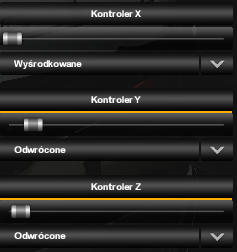
\includegraphics[width=6cm]{img/appendix1_controller.png}
  \caption{Poprawnie zidentyfikowany kontroler}
  \label{fig:appendix1_controller}
\end{figure}

\begin{figure}
  \centering
  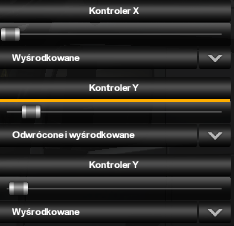
\includegraphics[width=6cm]{img/appendix1_bad_controller.png}
  \caption{Źle zidentyfikowana oś sterowania hamulcem}
  \label{fig:appendix1_bad_controller}
\end{figure}

Czasami, prawdopodobnie w wyniku błędu gry, oś odpowiedzialna za kontrolę hamulca nie jest poprawnie wykrywana (\ref{fig:appendix1_bad_controller}. Wtedy należy w ustawieniach kontrolera kliknąć na nazwę osi odpowiedzialną za hamulec i przy uruchomionej aplikacji wpisać:\\ \textsc{import time \\
time.sleep(10)\\
display2control.put([1, None, 100])\\
pass\\}

Zawsze w trakcie pracy aplikacji jest możliwość sterowania ciężarówką za pomocą klawiszy \textbf{W,S,A,D}, co jest przydatne na początku testowania algorytmów wizyjnych.

\section{Obsługa konsoli}
Konsola deweloperska zapewnia możliwość zmiany czasu gry, pogody, prędkości gry oraz lokalizacji. Użyteczne komendy:
\begin{itemize}
\item \textit{g\_ set\_ time hh} -- komenda zmieniająca czas gry, w miejsce \textit{hh} należy wpisać pożądaną godzinę
\item \textit{g\_ set\_ weather x} -- komenda zmieniająca pogodę. W miejsce \textit{x} można wpisać 1 lub 0 (słonecznie lub deszcz)
\item \textit{goto CITY} -- zmienia lokalizację. Później należy jeszcze przeteleportować ciężarówkę klawiszem F9.
\item \textit{warp x} --zmiana prędkości gry. \textit{X} to współczynnik prędkości. Wartości mniejsze od 1 zwalniają symulator, a wartości większe przyspieszają.
\end{itemize}

 \chapter{Zawartość płyty CD}
Zawartość płyty CD:
\begin{itemize}
\item Tekst pracy w postaci pliku PDF
\item Tekst pracy w postaci plików źródłowych Latexa
\item Aktualna wersja aplikacji w postaci skryptów Pythona
\end{itemize}
% itd.

\printbibliography

\end{document}
